\part{Results}
\label{pa:results}
\chapter{Ranklust as a tool for researchers}
\section{The planned workflow in general}
First off is the general workflow:
\begin{figure}[H]
    \label{fig:ranklust-workflow}
    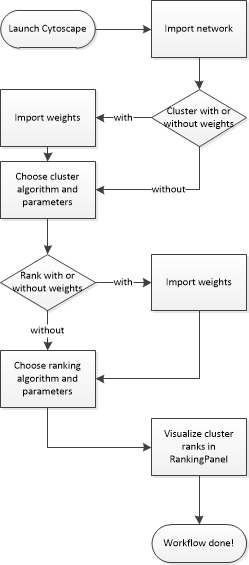
\includegraphics[scale=0.8]{ranklust_workflow}
\end{figure}

\section{Detailed walk-through of using Ranklust}
To go into more detail, here is the startup screen that the user is met with
after launching Cytoscape. This assumes that clusterMaker2 with the Ranklust
contribution is already installed into Cytoscape.
\begin{figure}[H]
    \label{fig:startup}
    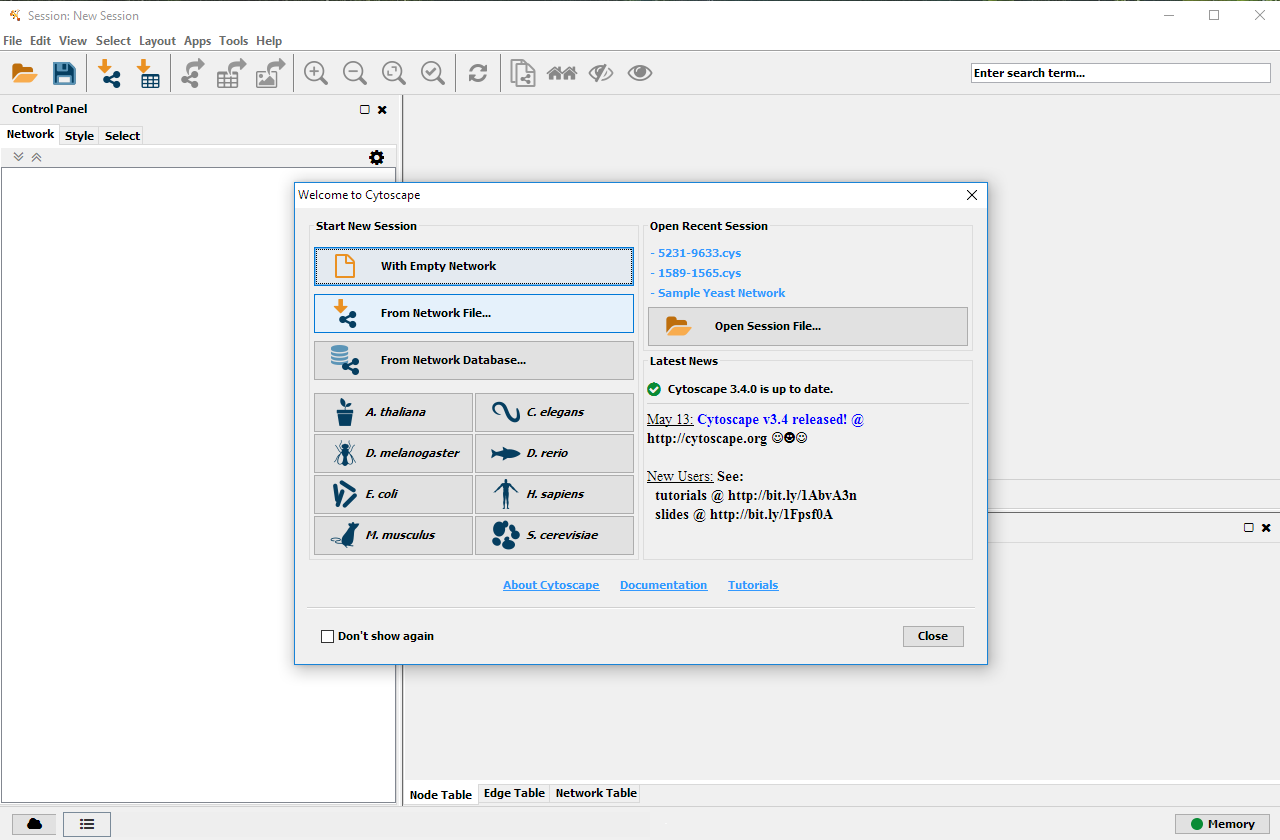
\includegraphics[width=15cm]{1-startup}
\end{figure}

This screen is what opens up after opting to import a network and choose a
network file consisting of a header that represents source and target node
columns, a\_alias and b\_alias.
\begin{figure}[H]
    \label{fig:import}
    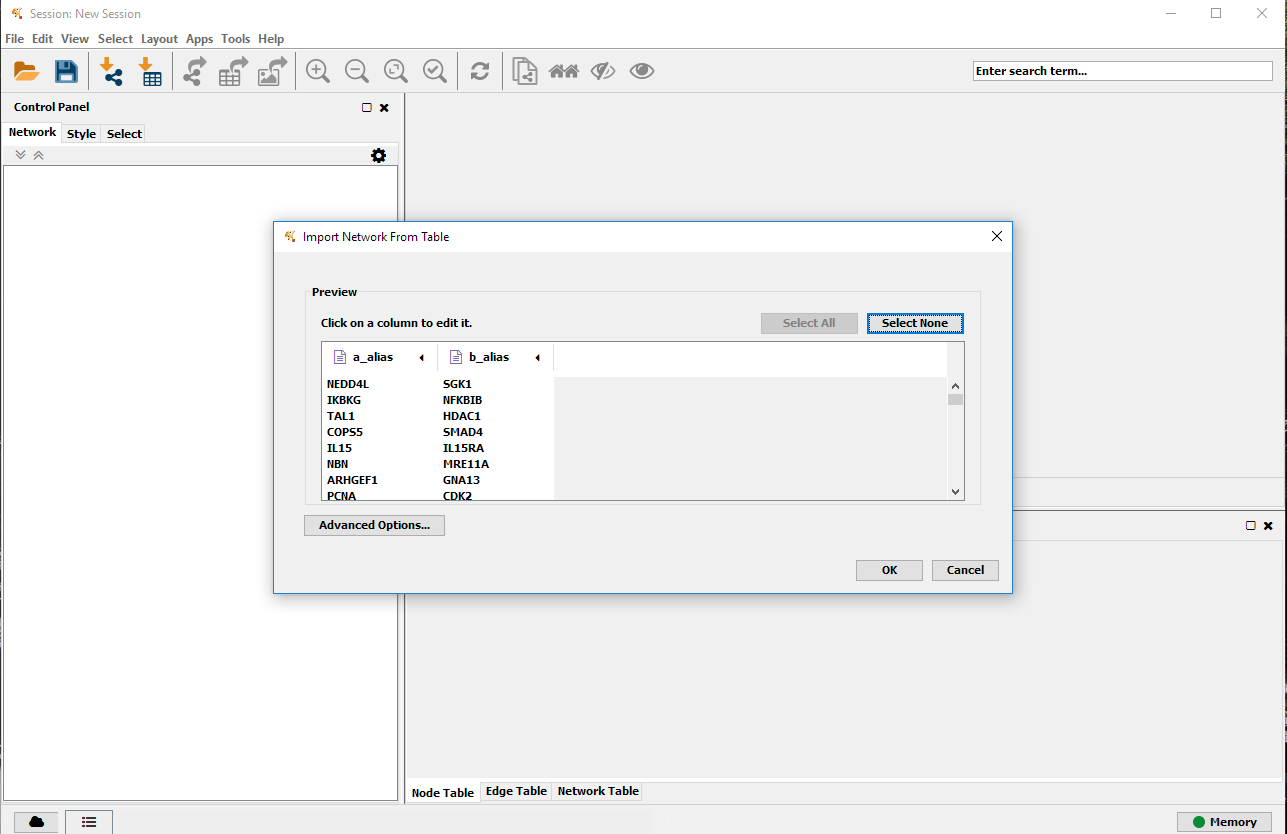
\includegraphics[width=15cm]{2-import}
\end{figure}

It is important to tell Cytoscape which column is considered as the source and
target column, as shown here. In this thesis, genes has been the primary key
identifier in both source and target column.
\begin{figure}[H]
    \label{fig:nodes}
    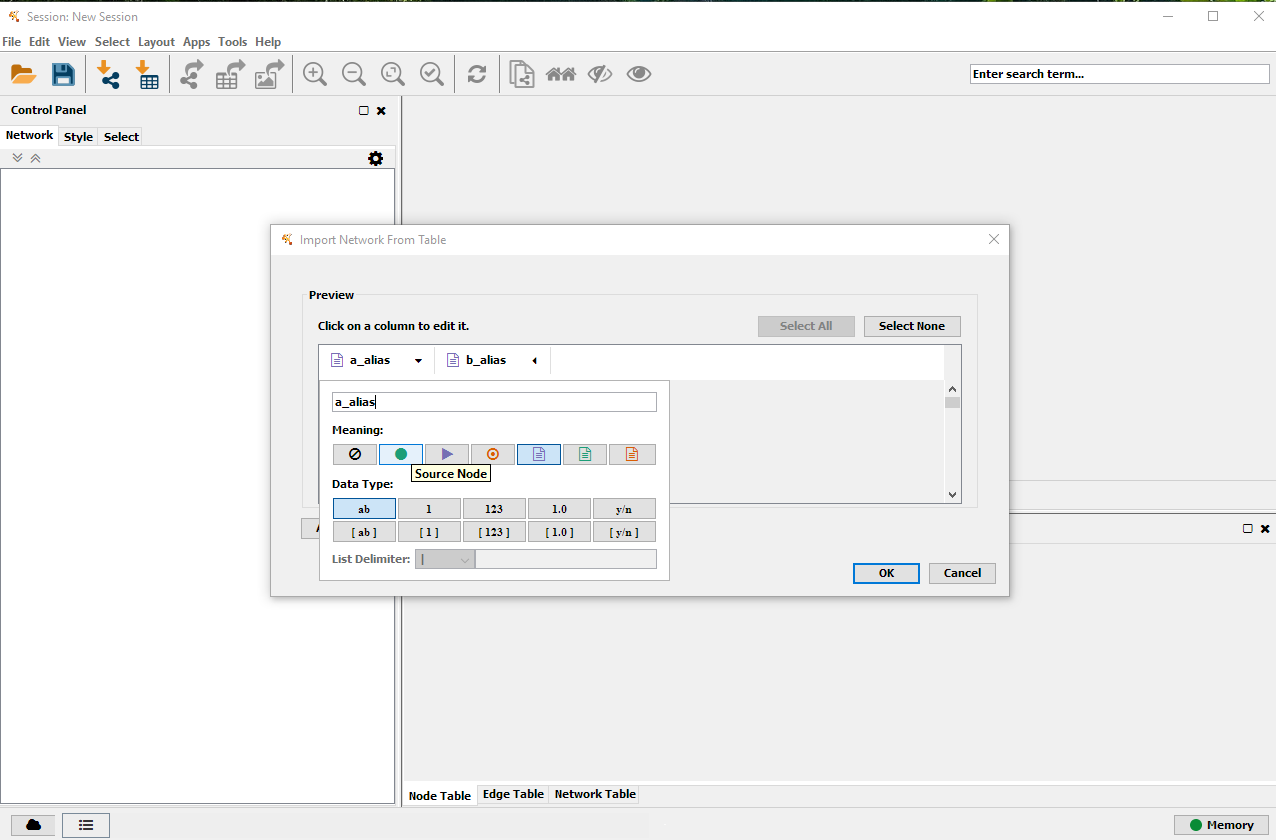
\includegraphics[width=15cm]{3-nodes}
\end{figure}

This is how Cytoscape looks after importing the network and it has finished its
standard style layout algorithm, which happens automatically after clicking "OK"
in the previous screen - having set everything to the correct settings.
\begin{figure}[H]
    \label{fig:imported-network}
    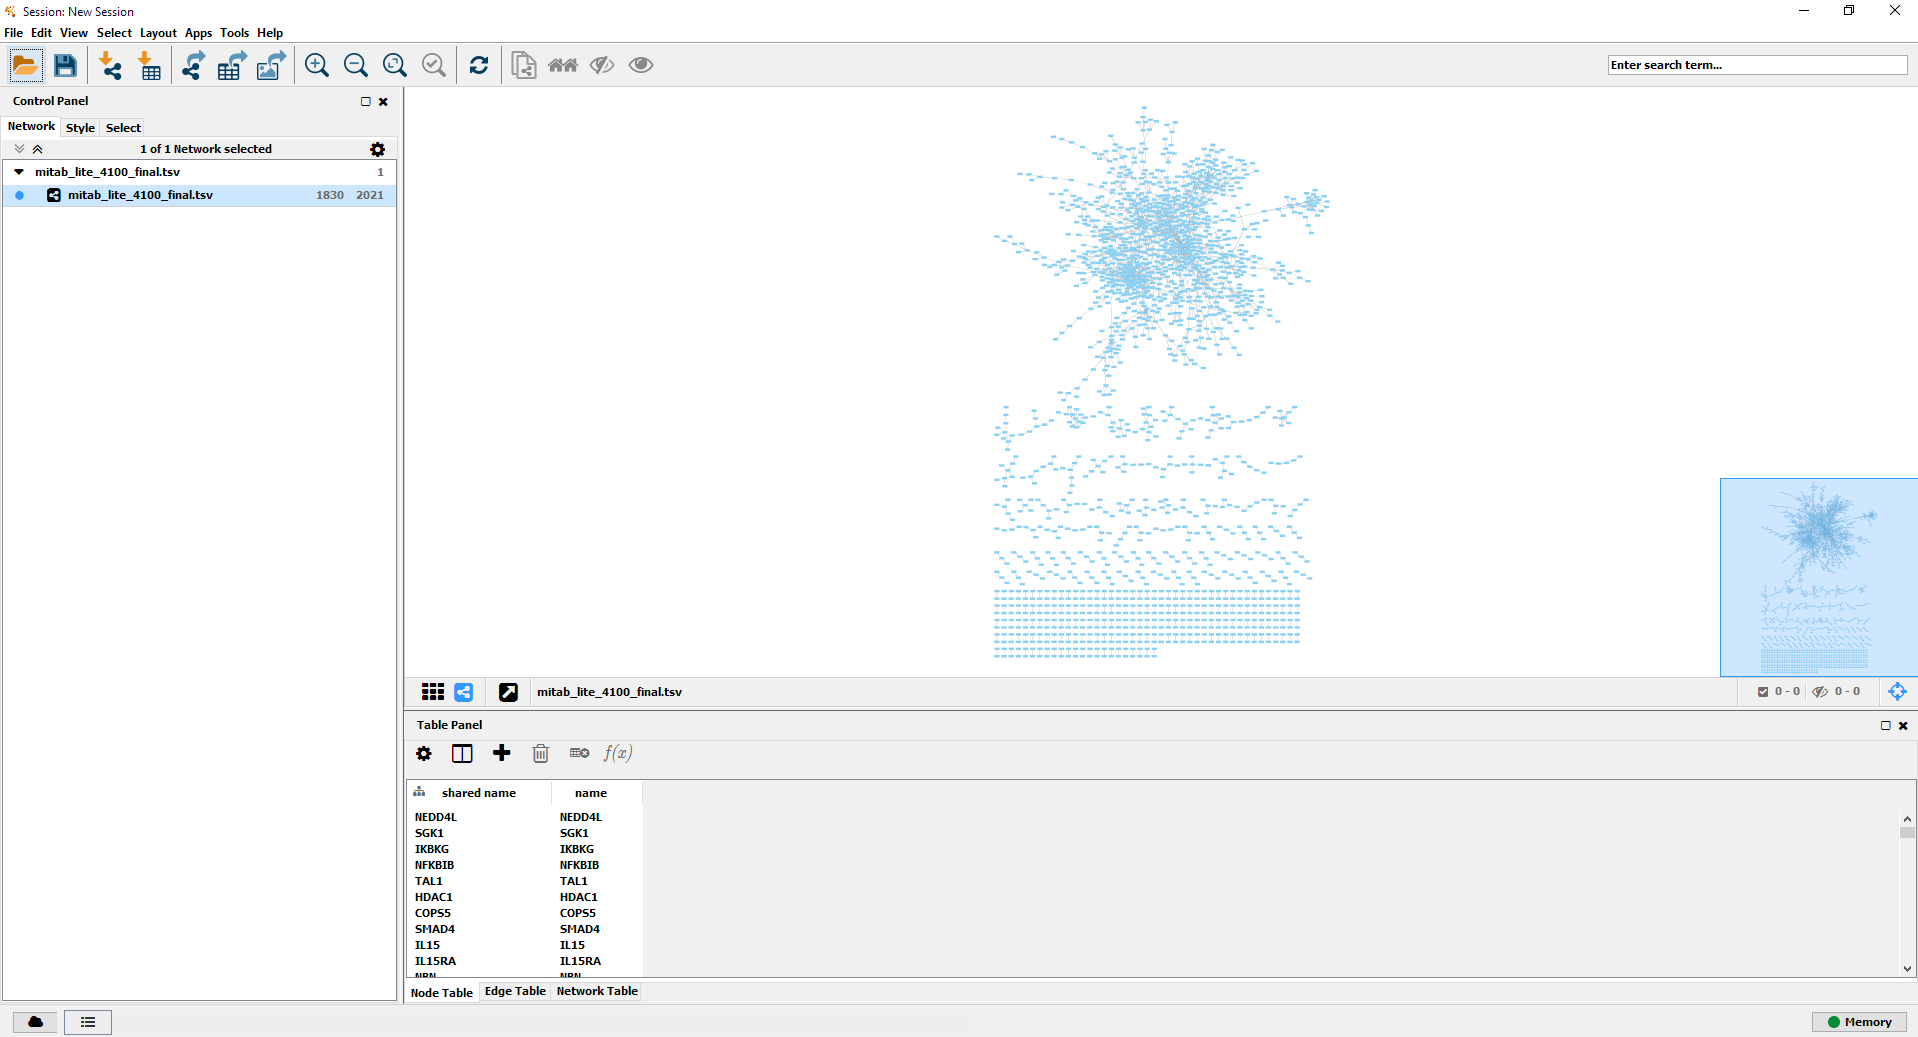
\includegraphics[width=15cm]{4-imported-network}
\end{figure}

If the user wishes to weight nodes for clustering or the ranking of them, it is
possible to do this with the "Import Columns From Table" function.
\begin{figure}[H]
    \label{fig:import-table}
    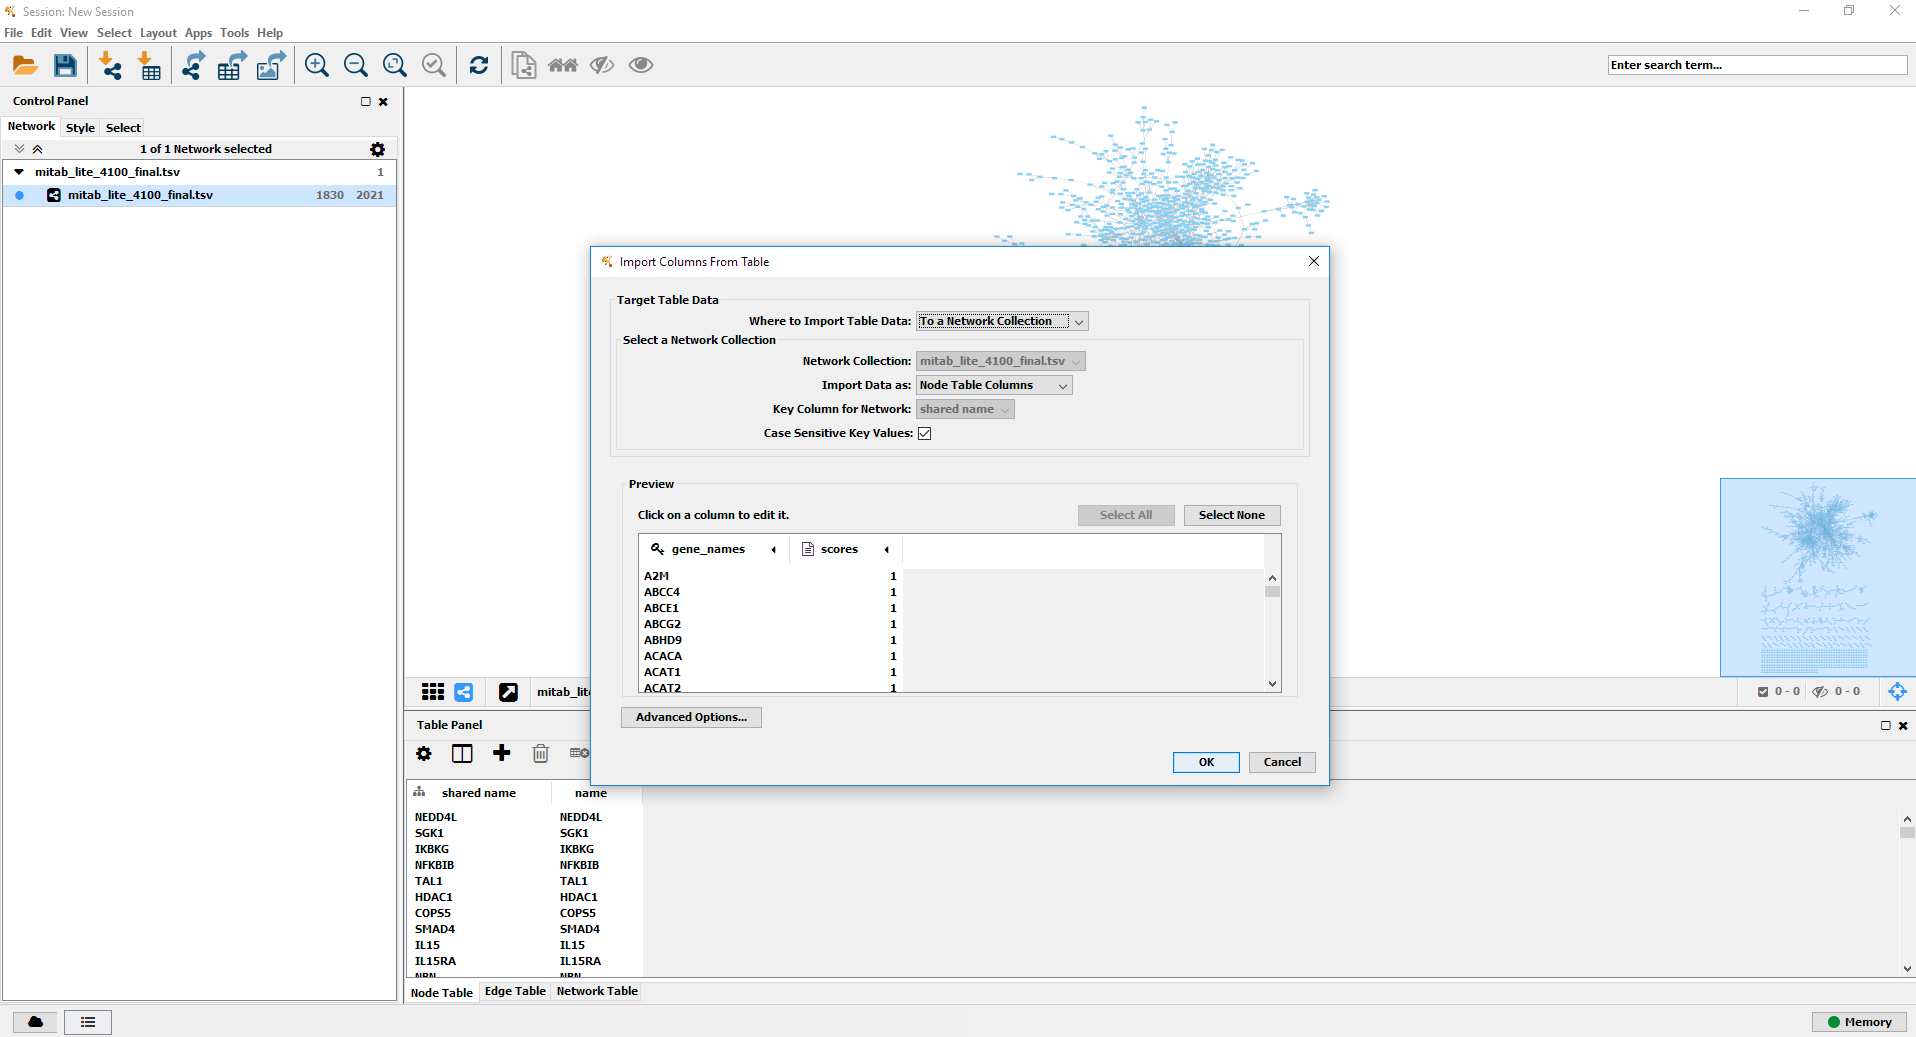
\includegraphics[width=15cm]{5-import-table}
\end{figure}

To cluster the network, the user has to access the \textit{Apps} menu at the top
in the toolbar of Cytoscape. In clusterMaker2 there are three rows belonging
to the plugin. \textit{clusterMaker}, where the clustering algorithms are
located. \textit{clusterMaker Ranking}, where the cluster ranking algorithms
\gls{maa},\gls{mam},\gls{pr},\gls{prwp} and \gls{hits} are. Finally, the
\textit{clusterMaker Visualizatons}, where different visualizations in
clusterMaker2 can be queried. This row is also where the visualizaton of the
ranked clusters option resides.
\begin{figure}[H]
    \label{fig:cluster}
    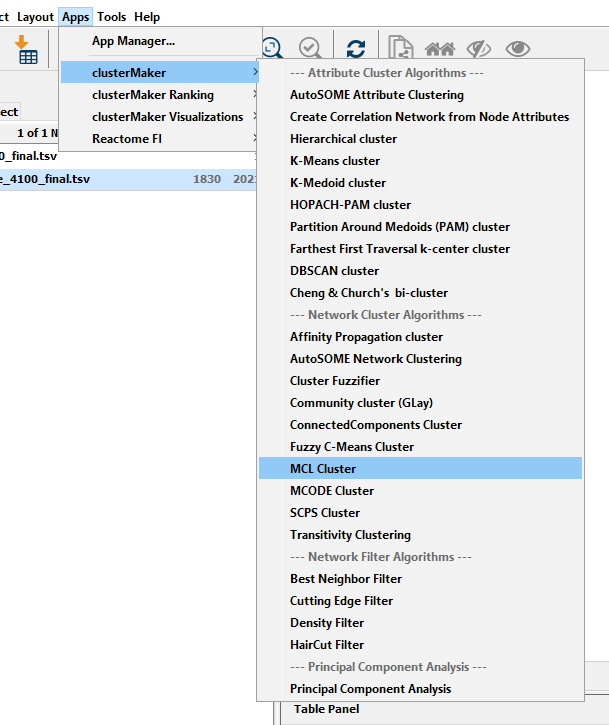
\includegraphics[width=15cm]{6-cluster}
\end{figure}

This is the view after clusterMaker2 has run the \textit{MCL cluster} method on
the current network. As seen on the left side menu, a new network has been
listed. This network only appears if the user sets the "Create new clustered
network"-option in the clustering parameter dialog that appears after choosing a
clustering algorithm from the clusterMaker2 menu.
\begin{figure}[H]
    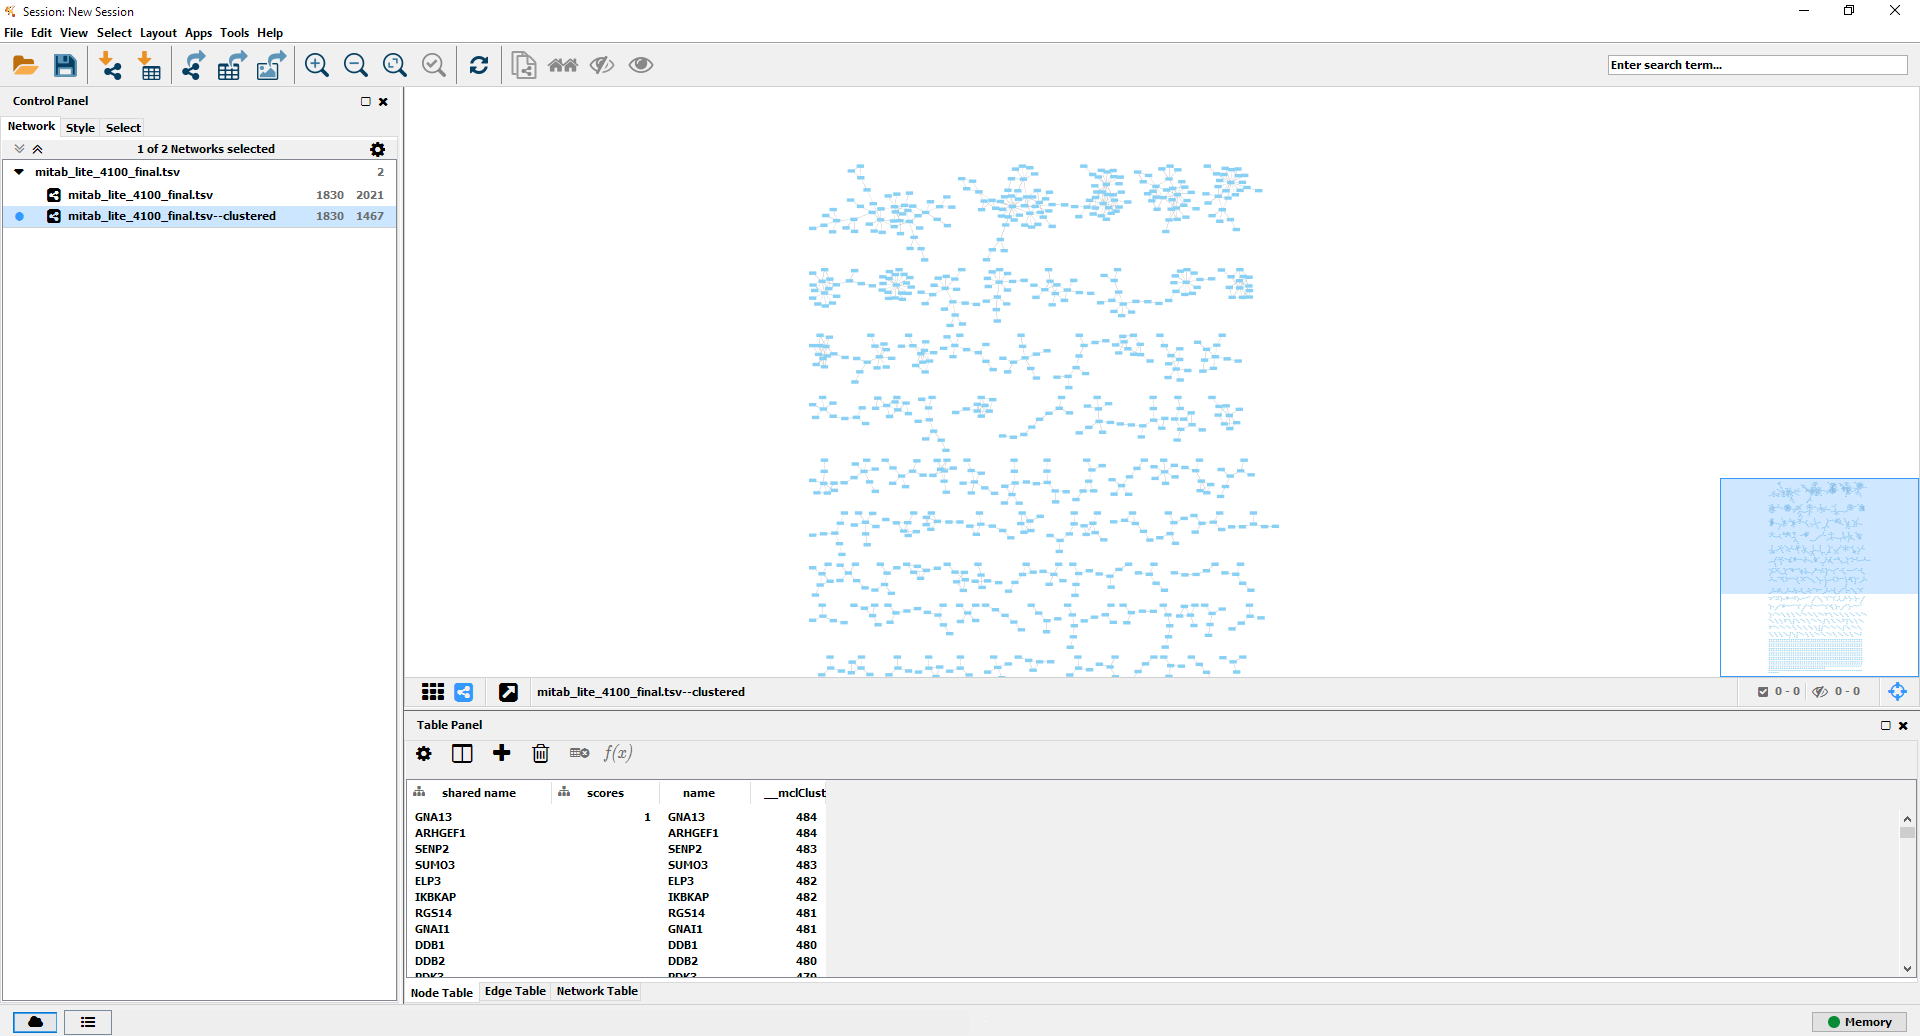
\includegraphics[width=15cm]{7-done-cluster}
    \label{fig:done-cluster}
\end{figure}

Here the cluster ranking algorithm menu is shown.
\begin{figure}[H]
    \label{fig:choose-ranking}
    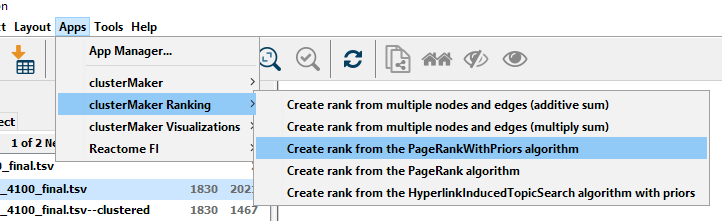
\includegraphics[width=15cm]{8-choose-ranking}
\end{figure}

The \gls{prwp} was chosen as the ranking algorithm. Node and edge attributes can
be combined by the user in any way. 
\begin{figure}[H]
    \label{fig:pagerank}
    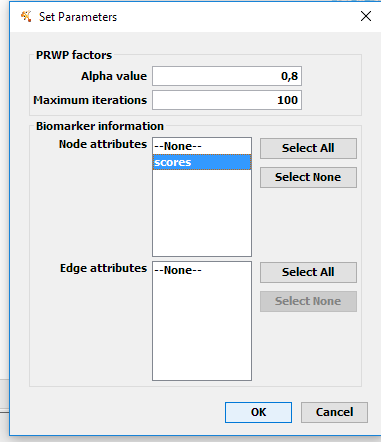
\includegraphics[width=15cm]{9-pagerank}
\end{figure}

If the user is interested in visualizing the ranks, it is possible to click the
"Show results from ranking clusters" option in the visualization menu. No menu
will appear after that, but rather will Cytoscape open a loading dialog similar
to when clustering and ranking algorithms has been tasked to start.
\begin{figure}[H]
    \label{fig:show-results}
    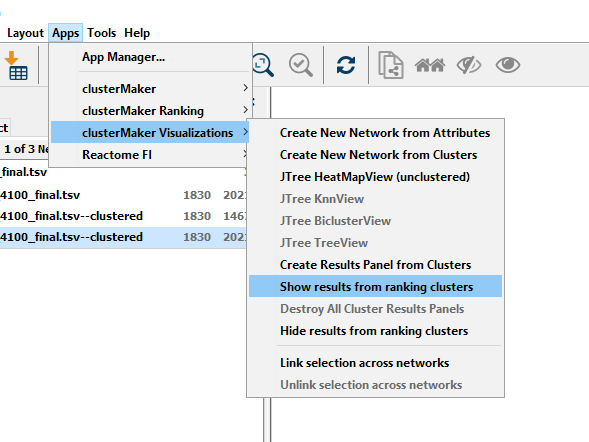
\includegraphics[width=15cm]{10-show-results}
\end{figure}

Here is the results panel displaying the ranked clusters from top to bottom,
descending scores. The title for each results panel is formatted as in the
example.
\begin{Verbatim}[fontsize=\scriptsize]
[<clustering algorithm>]{<ranking algorithm>}(<network name>)
\end{Verbatim}
So with MCL clustering, \gls{prwp} ranking and the
"mitab\_lite\_4100\_final.tsv--clustered" network, this is what the title
becomes:
\begin{Verbatim}[fontsize=\scriptsize]
[mcl]{PRWP}(mitab_lite_4100_final.tsv--clustered)
\end{Verbatim}
As seen in the title. The coloring has been discussed earlier.
\begin{figure}[H]
    \label{fig:result-colors}
    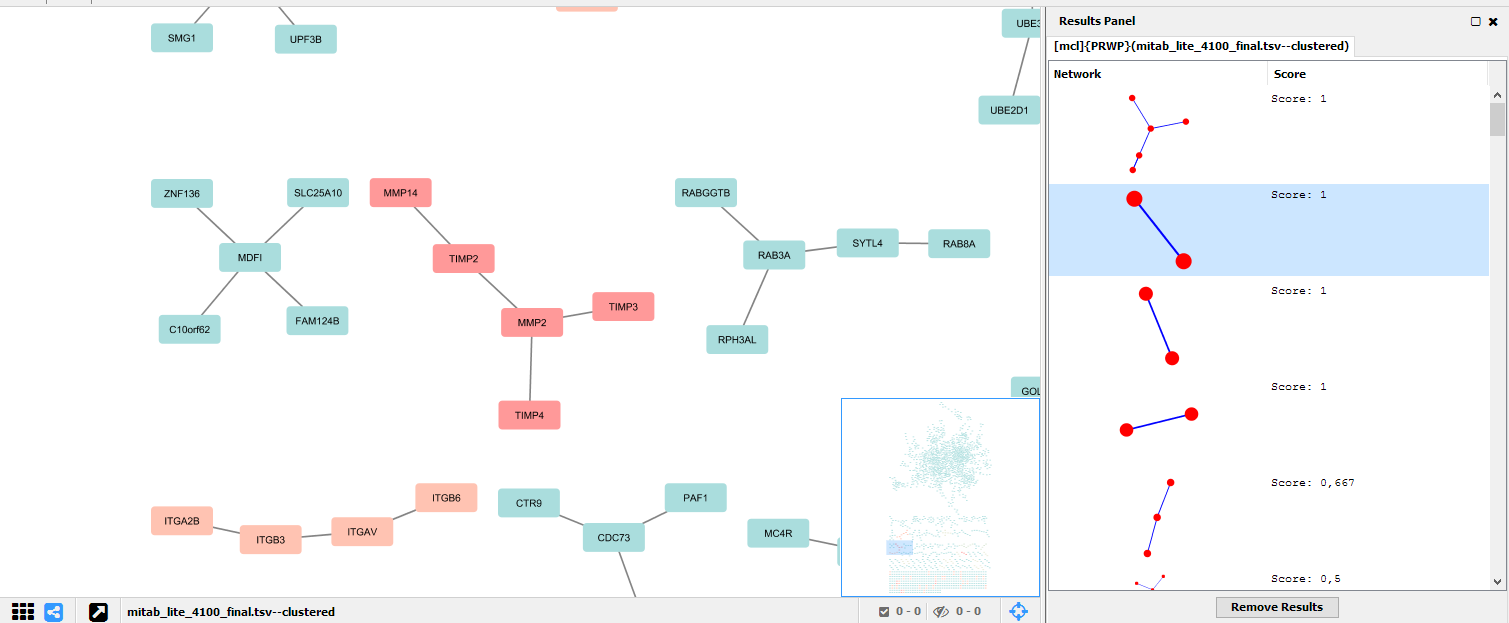
\includegraphics[width=15cm]{11-result-colors}
\end{figure}

Here is an example of how the clusters change color when selected from the
results panel menu.
\begin{figure}[H]
    \label{fig:rank-selection}
    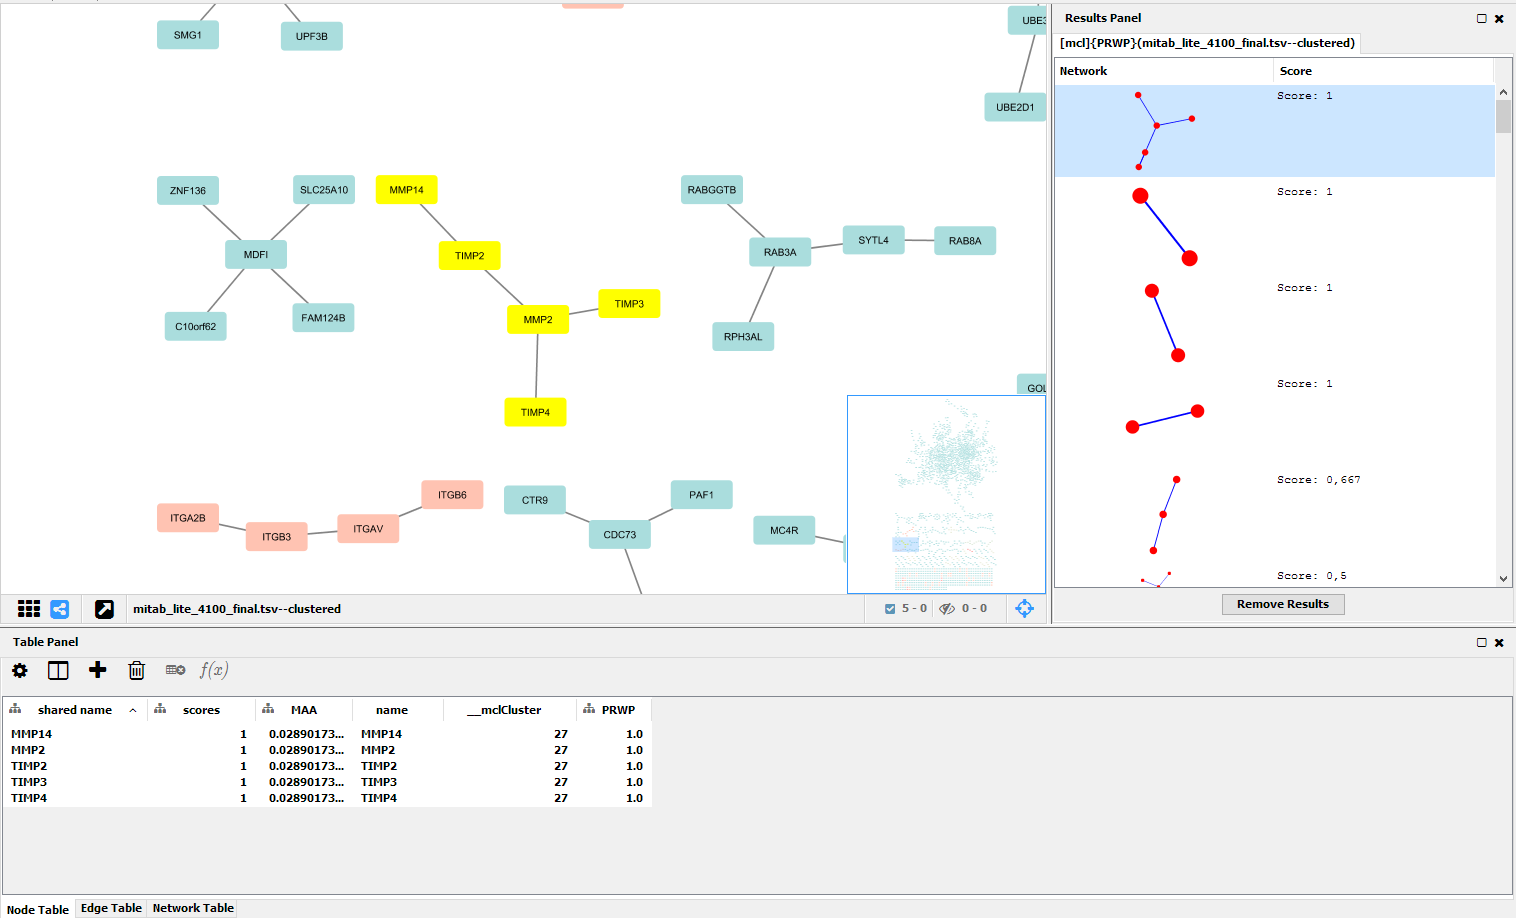
\includegraphics[width=15cm]{12-rank-selection}
\end{figure}

\section{Design}
\begin{figure}[H]
    \caption{Ranklust ranking algorithm relations}
    \label{fig:rank-alg}
    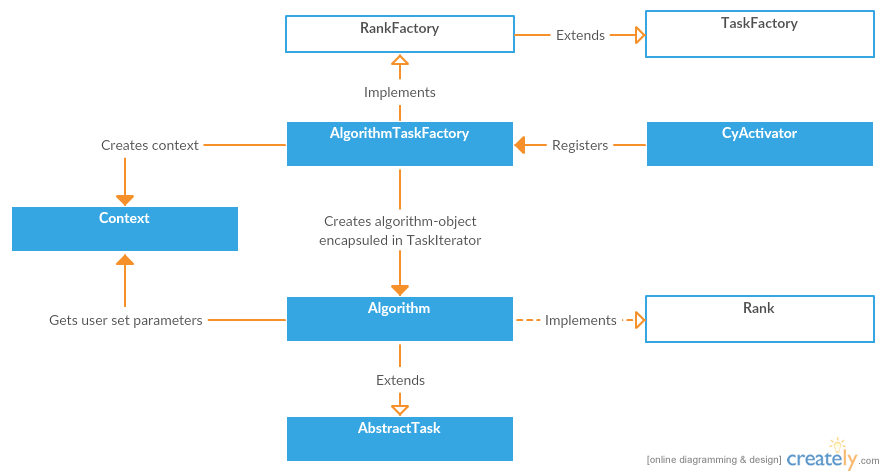
\includegraphics[width=\textwidth]{ranklust-algorithm}
\end{figure}
\begin{figure}[H]
    \caption{Ranklust ranking panel relations}
    \label{fig:rank-panel}
    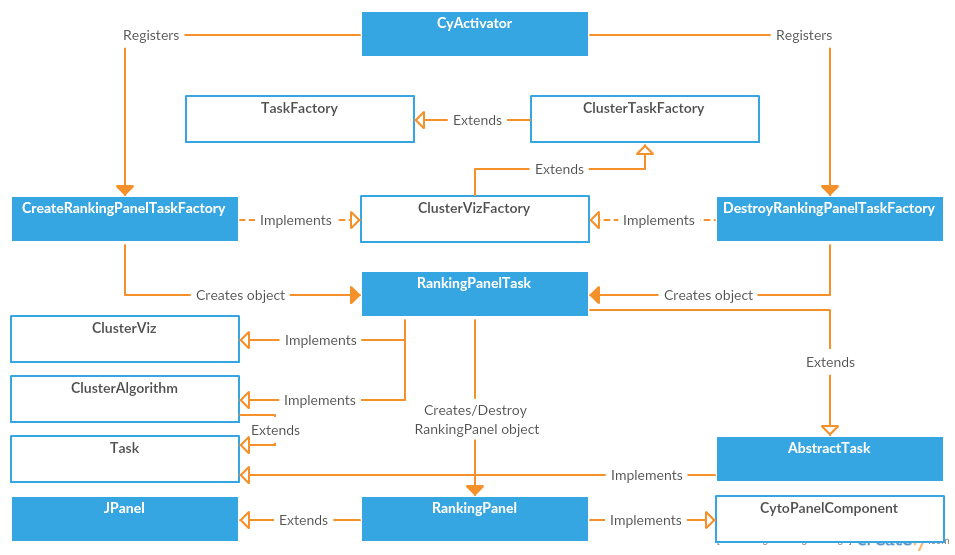
\includegraphics[width=\textwidth]{ranklust-panel}
\end{figure}

\chapter{Graph analysis}
\section{Creating the network}
After querying iRefWeb for the PPI-network with the query displayed earlier
(\ref{fig:irefweb}) the resulting network consisted of 109276 interactions.
After filtering the same network through the protein-to-gene mapping constructed
from HGNC, the final network consisted of 9500 nodes (genes) and 43706 edges
(interactions). At this point, all of the nodes and edges were undirected and
unweighted. Converting from proteins to genes ended up with a 60\% perturbation
of the network in the form of removed edges. Clustering the network resulted in
a further perturbation of 69.8\% of edge-removal when compared to the
HGNC-filtered network, 87.9\% when compared to the unfiltered iRefWeb network.

The creation of the \gls{golden} through combining DisGeNET and \gls{dragon}
resulted in a file with two columns. One representing a gene, the second one
representing the score of a gene, so a single row would contain a unique gene in
the list and the score it received.

\section{Ranking results}
Talking about \gls{mcl} results
\hspace*{-2cm}\begin{table}[H]
    \centering
    \begin{tabular}{| l | c | c | c | c | c | c |}
        \hline
        \textbf{Inflation} & \textbf{Clusters} & \textbf{Avg.  cluster size} &
        \textbf{Max. cluster size} & \textbf{Min. cluster size} &
        \textbf{Modularity} \\
        \hline
        1.6 & 1068 & 8.88 & 968 & 2 & 0.367 \\
        1.8 & 1400 & 6.60 & 660 & 2 & 0.307 \\
        2.0 & 1599 & 5.68 & 405 & 2 & 0.269 \\
        2.5 & 2053 & 4.20 & 179 & 2 & 0.223 \\
        3.0 & 2210 & 3.75 & 122 & 2 & 0.199 \\
        \hline
    \end{tabular}
    \caption{MCL clustering parameter and statistic results}
    \label{tab:mcl-inflation}
\end{table}
The modularity of the clustered networks gives an indicator of how well the
process of creating the clusters went. Modularity is given as a score from 0 to
1. A score closer to 1 is more preferrable, as this indicates that the clusters
created have a good degree of separation to the other clusters in the network.
The preferred score to end up with would be around 0.8, but in this network
there has been a good amount of perturbation through the protein-to-gene
process. Modularity is not the only indicator of how well a network was
clustered, hence the choice of not setting the inflation value in \gls{mcl} to
1.6, but rather 1.8. When a lower inflation value is set, \gls{mcl} does not
separate edges between nodes as vigorously and as a direct cause, inflation will
go up. Taking the other attributes in the table (\ref{tab:mcl-inflation}) into
consideration, 1.8 seemed like the best inflation value. An inflation value of
1.8 has also been proved to be good for large high-throughput constructed
protein-protein networks with a large amount of alterations\cite{mcl-inflation}.

The amount of iterations used for \gls{mcl} ended up being 200. It started out
at 1000, but the results converged somewhere between 170 and 200 iterations, so
it was decreased form 1000 to 200 to speed up the time used in the
\gls{pipeline}.

\section{Cross-validation}
Executing a cross-validation on the iRefWeb with PRWP and MAA rankings had two
purposes. The first being to prove the fact that every gene that had its prior
score removed by the cross-validation, should be found in the results of the
cluster ranking and identified as candidate biomarkers. 

The second purpose was to analyze the distribution of the genes with prior
scores removed by the cross-validation in terms of how they placed in the
cluster ranking. The analysis of this distribution was done by dividing the
amount of genes removed by cross-validation in a cluster by the total amount of
genes in the same cluster. This operation was repeated for every cluster in the
ranking, resulting in a distribution of the average amount of genes removed by
cross-validation, that was detected by Ranklust together with post-processing of
data, as cancer candidate biomarkers. A distinct descending distribution from
high to low ranked clusters would indicate that most of the genes, with a prior
score of their relevance to prostate cancer, was ranked in a way that achieved
the goal of Ranklust; ranking clusters in biological network according to
network structure and prior knowledge of relevance to diseases.

\subsection{Cross-validation in PRWP}
\hspace*{-2cm}\begin{figure}[H]
    \label{fig:irefweb-prwp}
    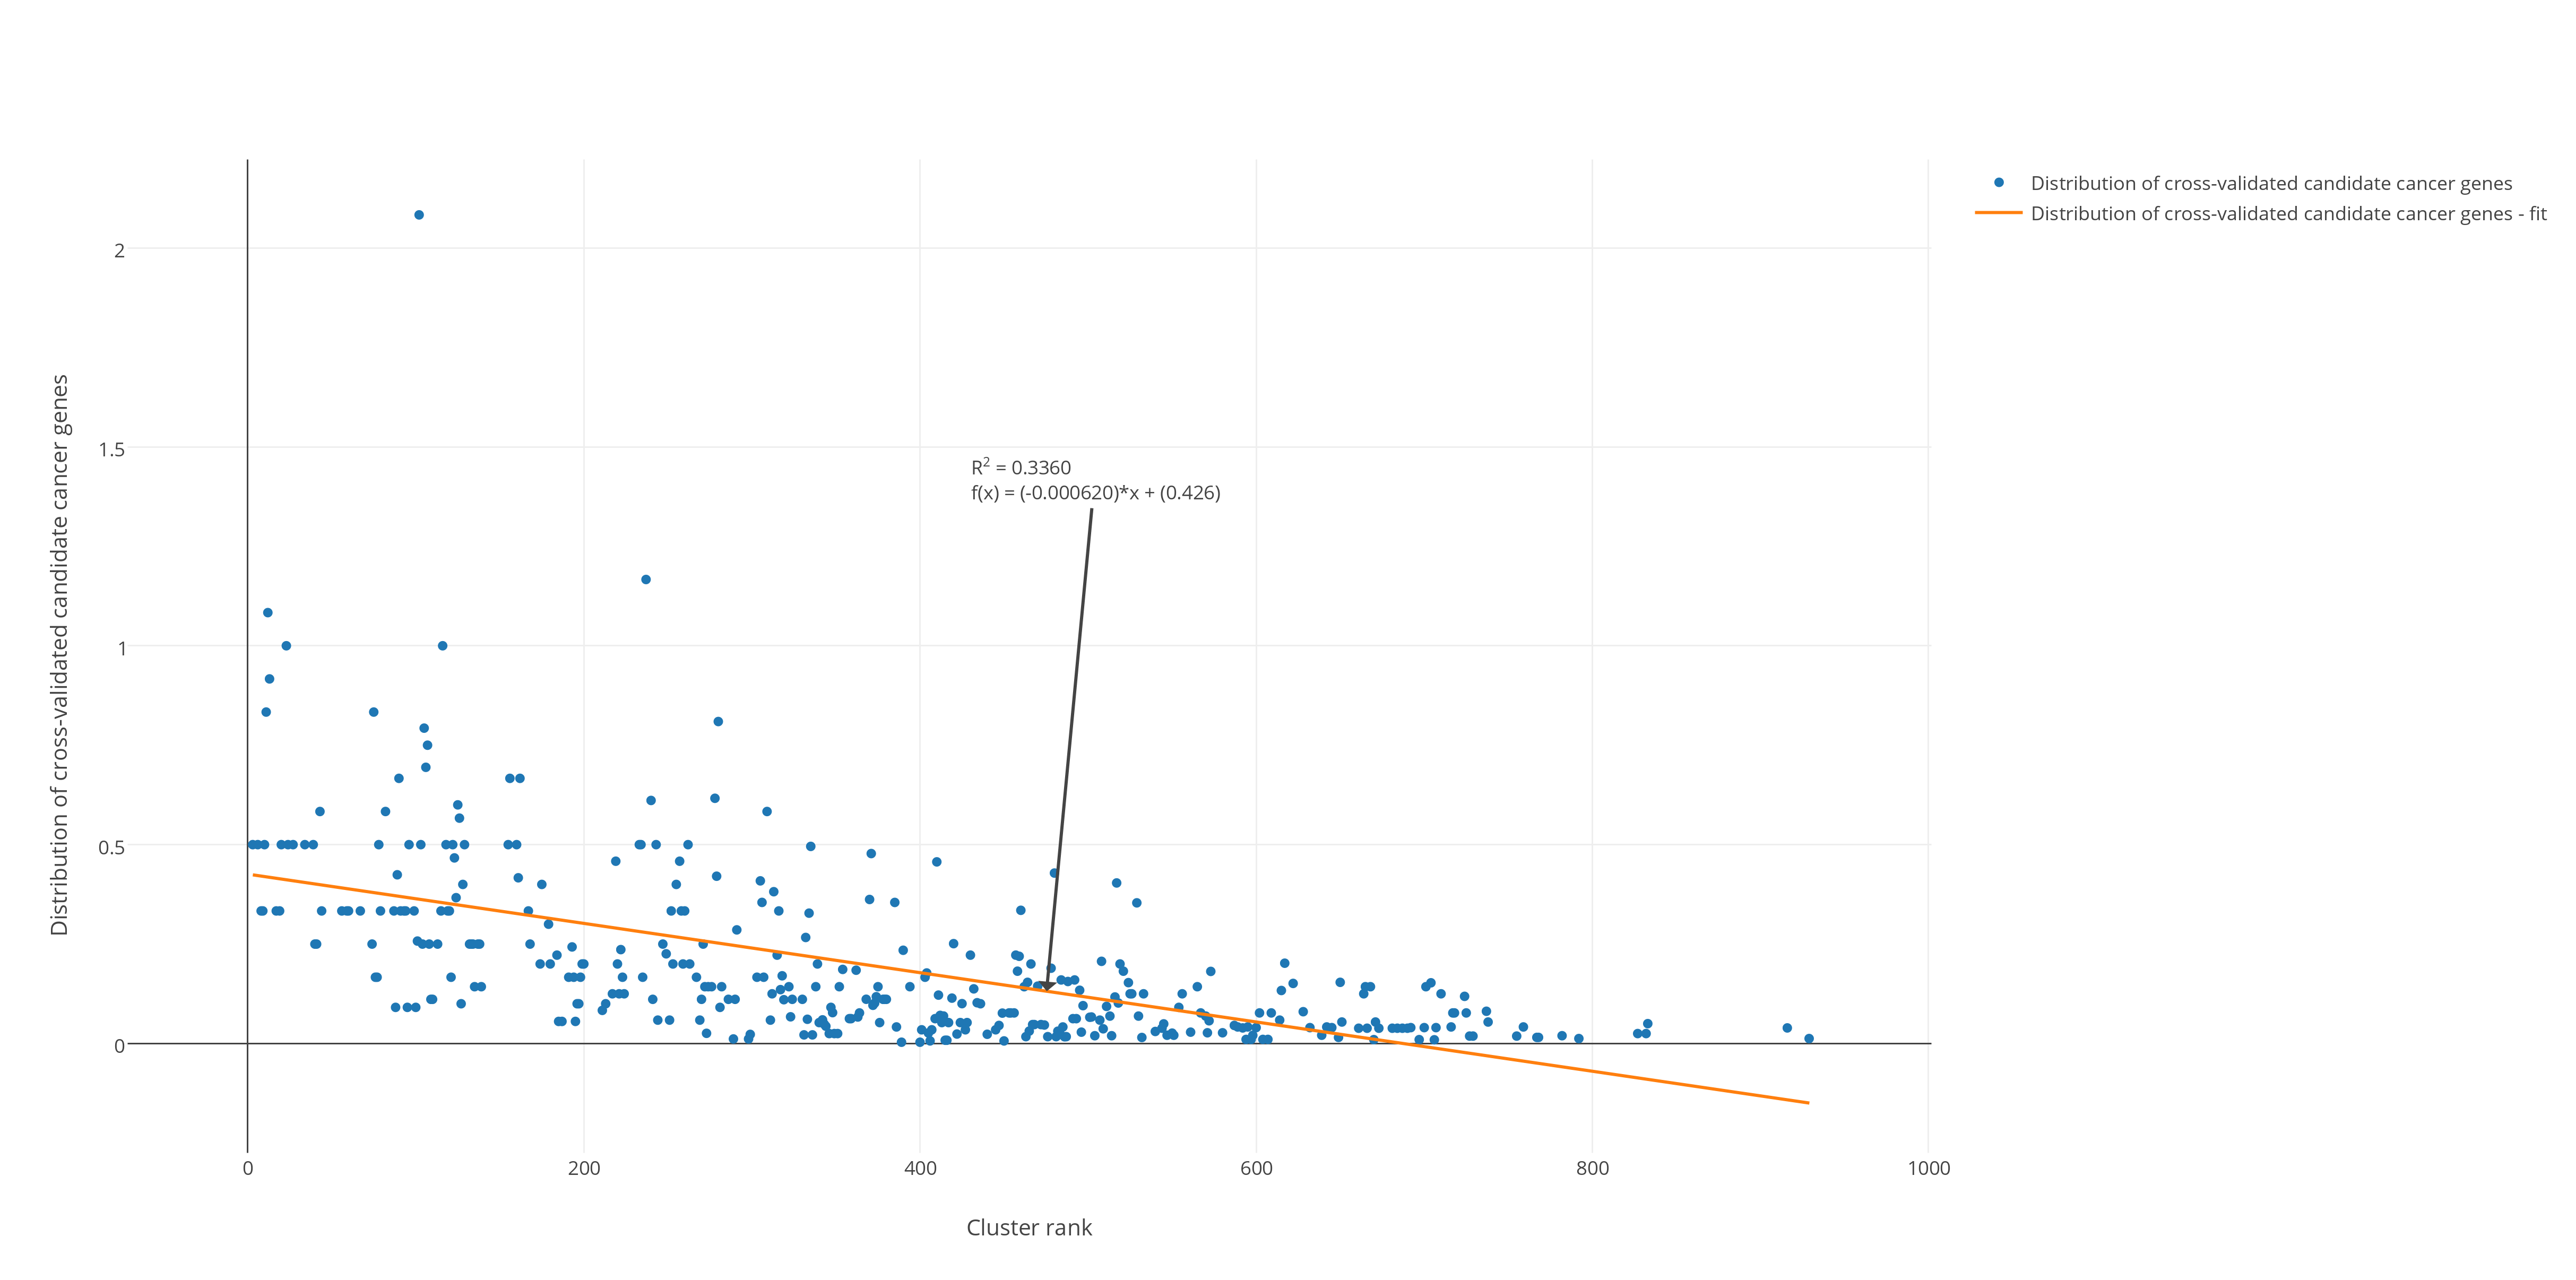
\includegraphics[scale=0.6]{cv_dist_total_filtered_prwp}
    \caption{Cross-validation distribution in clusters (PRWP)}
\end{figure}
This plot \ref{fig:irefweb-prwp} is developed from the 10 random
cross-validation runs ranked with PRWP. The results from this cross-validation
shows that the higher the rank of the cluster, the more candidate cancer genes
the cluster had.

\subsection{Cross-validation in MAA}
\hspace*{-2cm}\begin{figure}[H]
    \label{fig:irefweb-maa}
    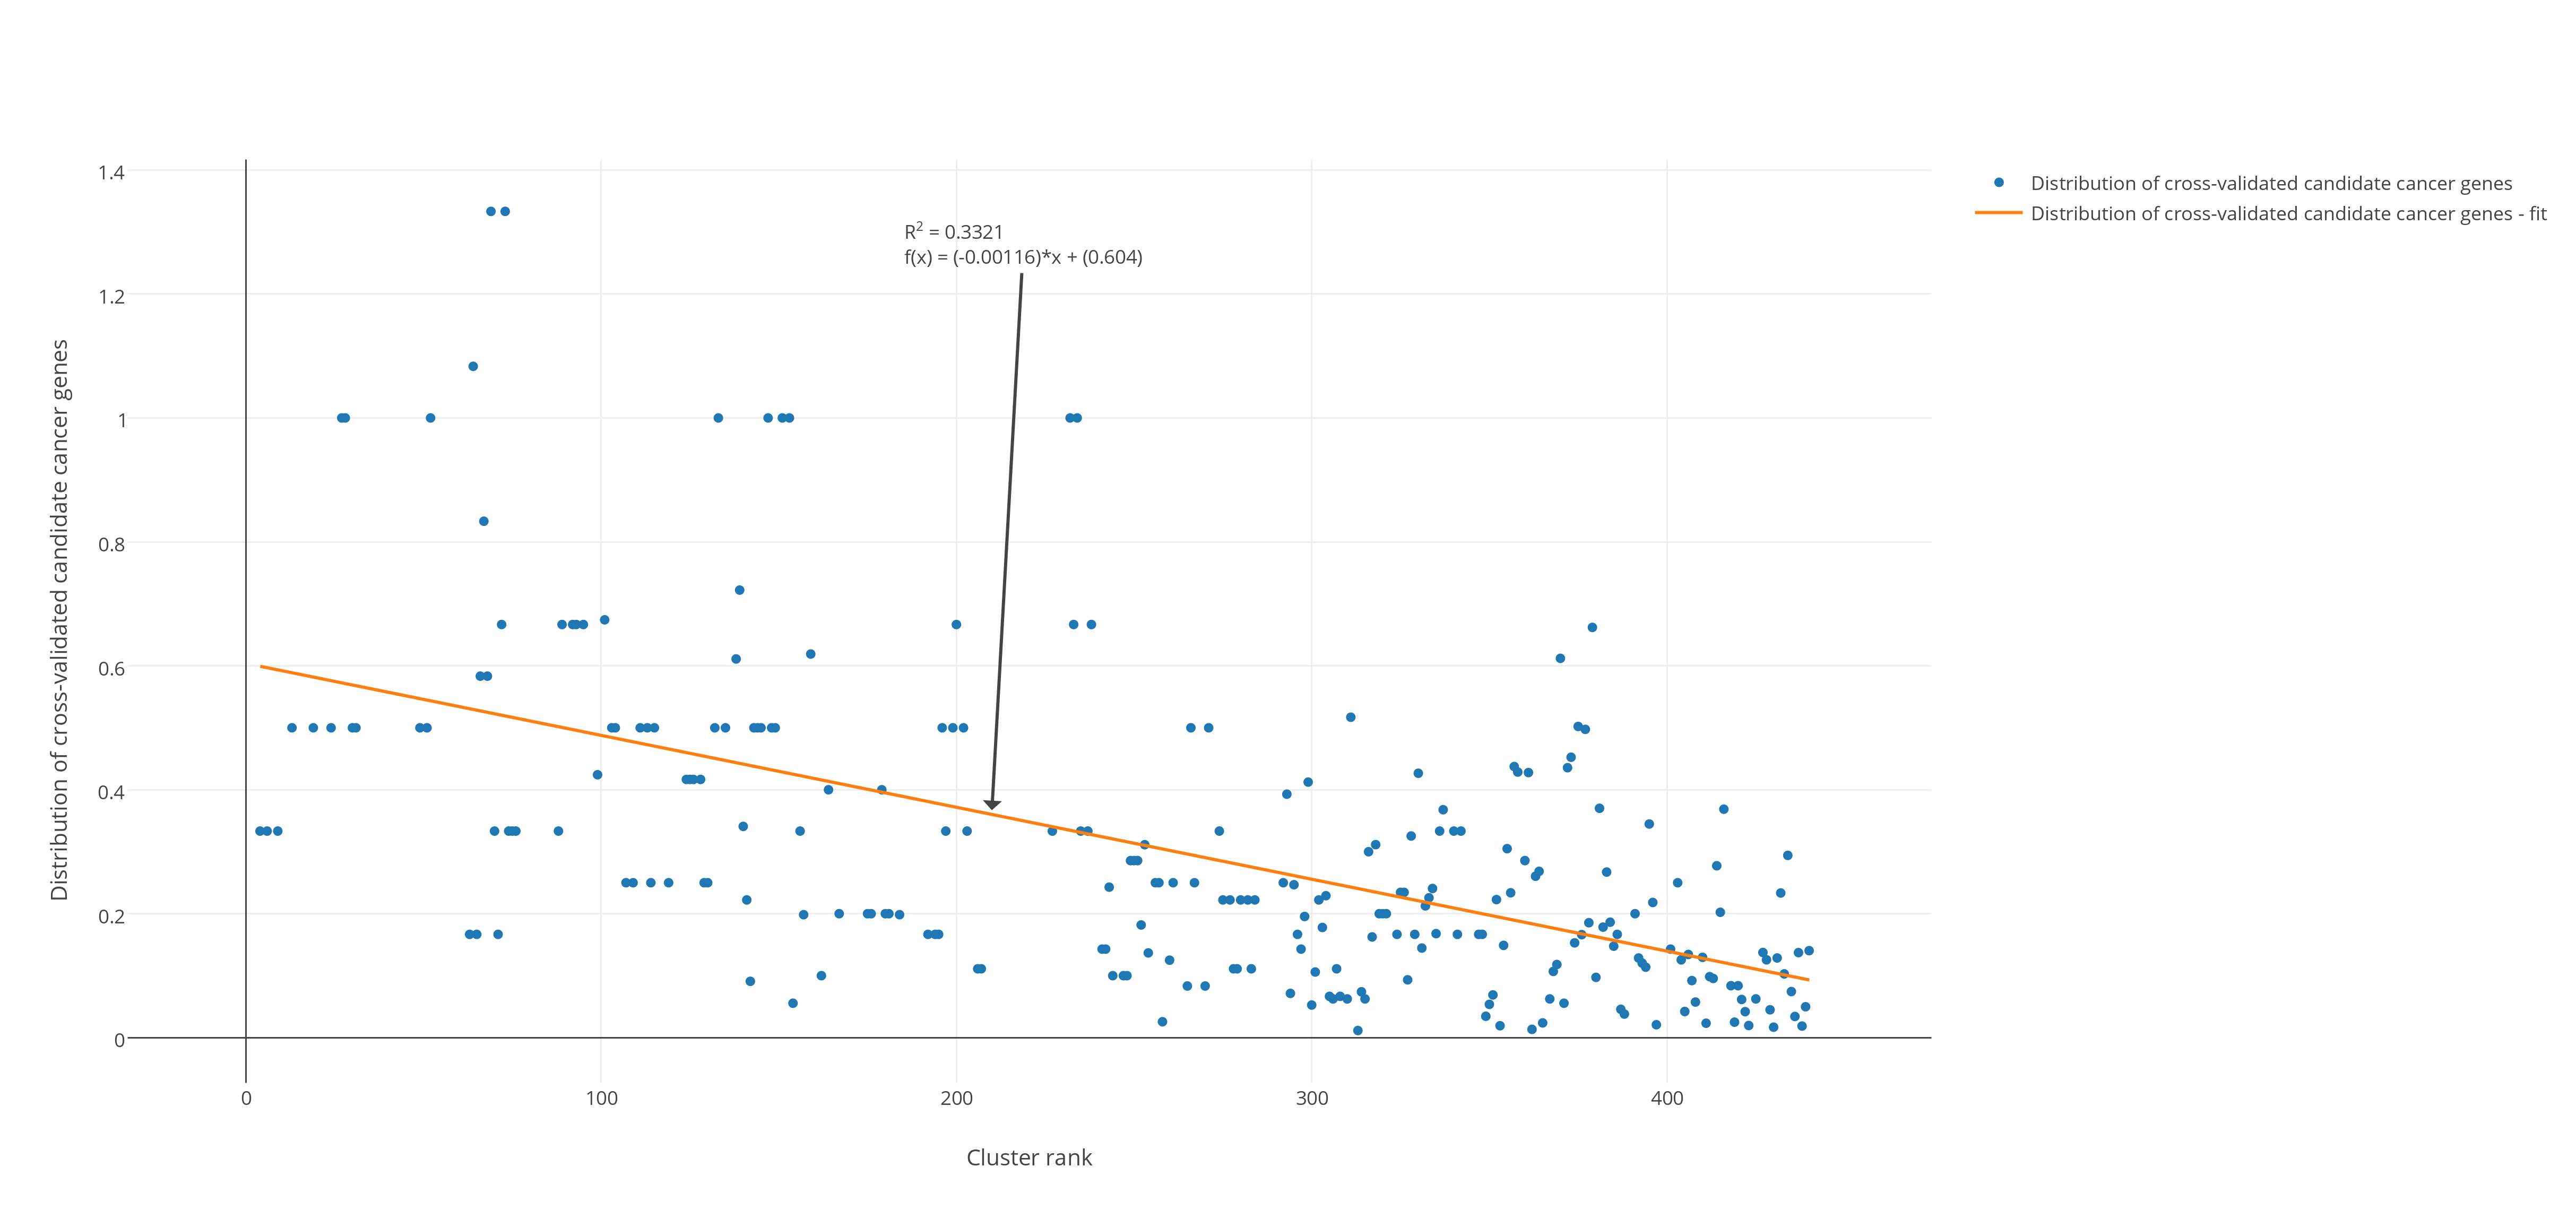
\includegraphics[scale=0.6]{cv_dist_total_filtered_maa}
    \caption{Cross-validation distribution in clusters (MAA)}
\end{figure}
This plot \ref{fig:irefweb-maa} is developed from the 10 random
cross-validatioon runs ranked with MAA. The results from this cross-validation
shows that the higher the rank of the cluster, the more candidate cancer genes
the cluster had.

\subsection{PRWP versus MAA}
There is clearly a trend in both \gls{prwp} and \gls{maa}. The difference
between them being mainly the amount of clusters found and the coupling of
values around the linear regression fit. It is important to point out that this
is just a result over the distribution of candidate cancer genes at certain
ranks. Where the clusters resides in the rankings may be very different between
the \gls{prwp} and \gls{maa}.

The fact that both of the ranking algorithms managed to get a descending amount
of prostate candidate cancer genes in the clusters, which was cross-validated
from the same \gls{golden} priors, indicates that a certain similarity of what
was mentioned in the previous paragraph. The similarity implicated here is how
different the ranking of the clusters are between \gls{prwp} and \gls{maa}.

The values in \gls{prwp} have a tighter coupling, in other words, the distance
the coordinates have in the scatter plot deviate less from the fit than the ones
in the \gls{maa} plot. The difference is not huge, as the coefficient of
determination indicates, 0.336 in \gls{prwp} against 0.332 in \gls{maa}. Both
ranking algorithms achieves a descending distribution of cross-validated genes
from the topmost to the lowest ranked cluster. But when comparing the
cross-validation results between \gls{prwp} and \gls{maa}, \gls{prwp} comes out
ahead by a margin in \gls{rsquared} value.

\section{Benchmarking Ranklust against biomarker resources}
In all of the upcoming plots of benchmarks, blue will represent prostate cancer
biomarkers from the \gls{golden} and orange represent prostate candidate cancer
biomarkers. The benchmarks are all based on prostate cancer data queried from
the \gls{jensen} database\cite{jensen}. The database has a hierarchy based
definition of diseases, so filtering the data on an insensitive-case "prostate
cancer"-query with the UNIX grep tool\cite{grep} retrieved all of the genes used
for the benchmark.

The average z-values in the clusters are split among 2 categories as mentioned
above. The z-values of the prostate candidate cancer genes in a cluster is
calculated from the average of all of them. The same procedure was done for the
z-values of the prostate cancer genes. 

The average knowledge curated genes...

The average p-values in the cluster...

\subsection{Text mined and scored with z-values}
These next z-value scored plots represents text mined gene results from the
\gls{jensen} database.

\begin{figure}[H]
    \label{fig:txt-iref-prwp}
    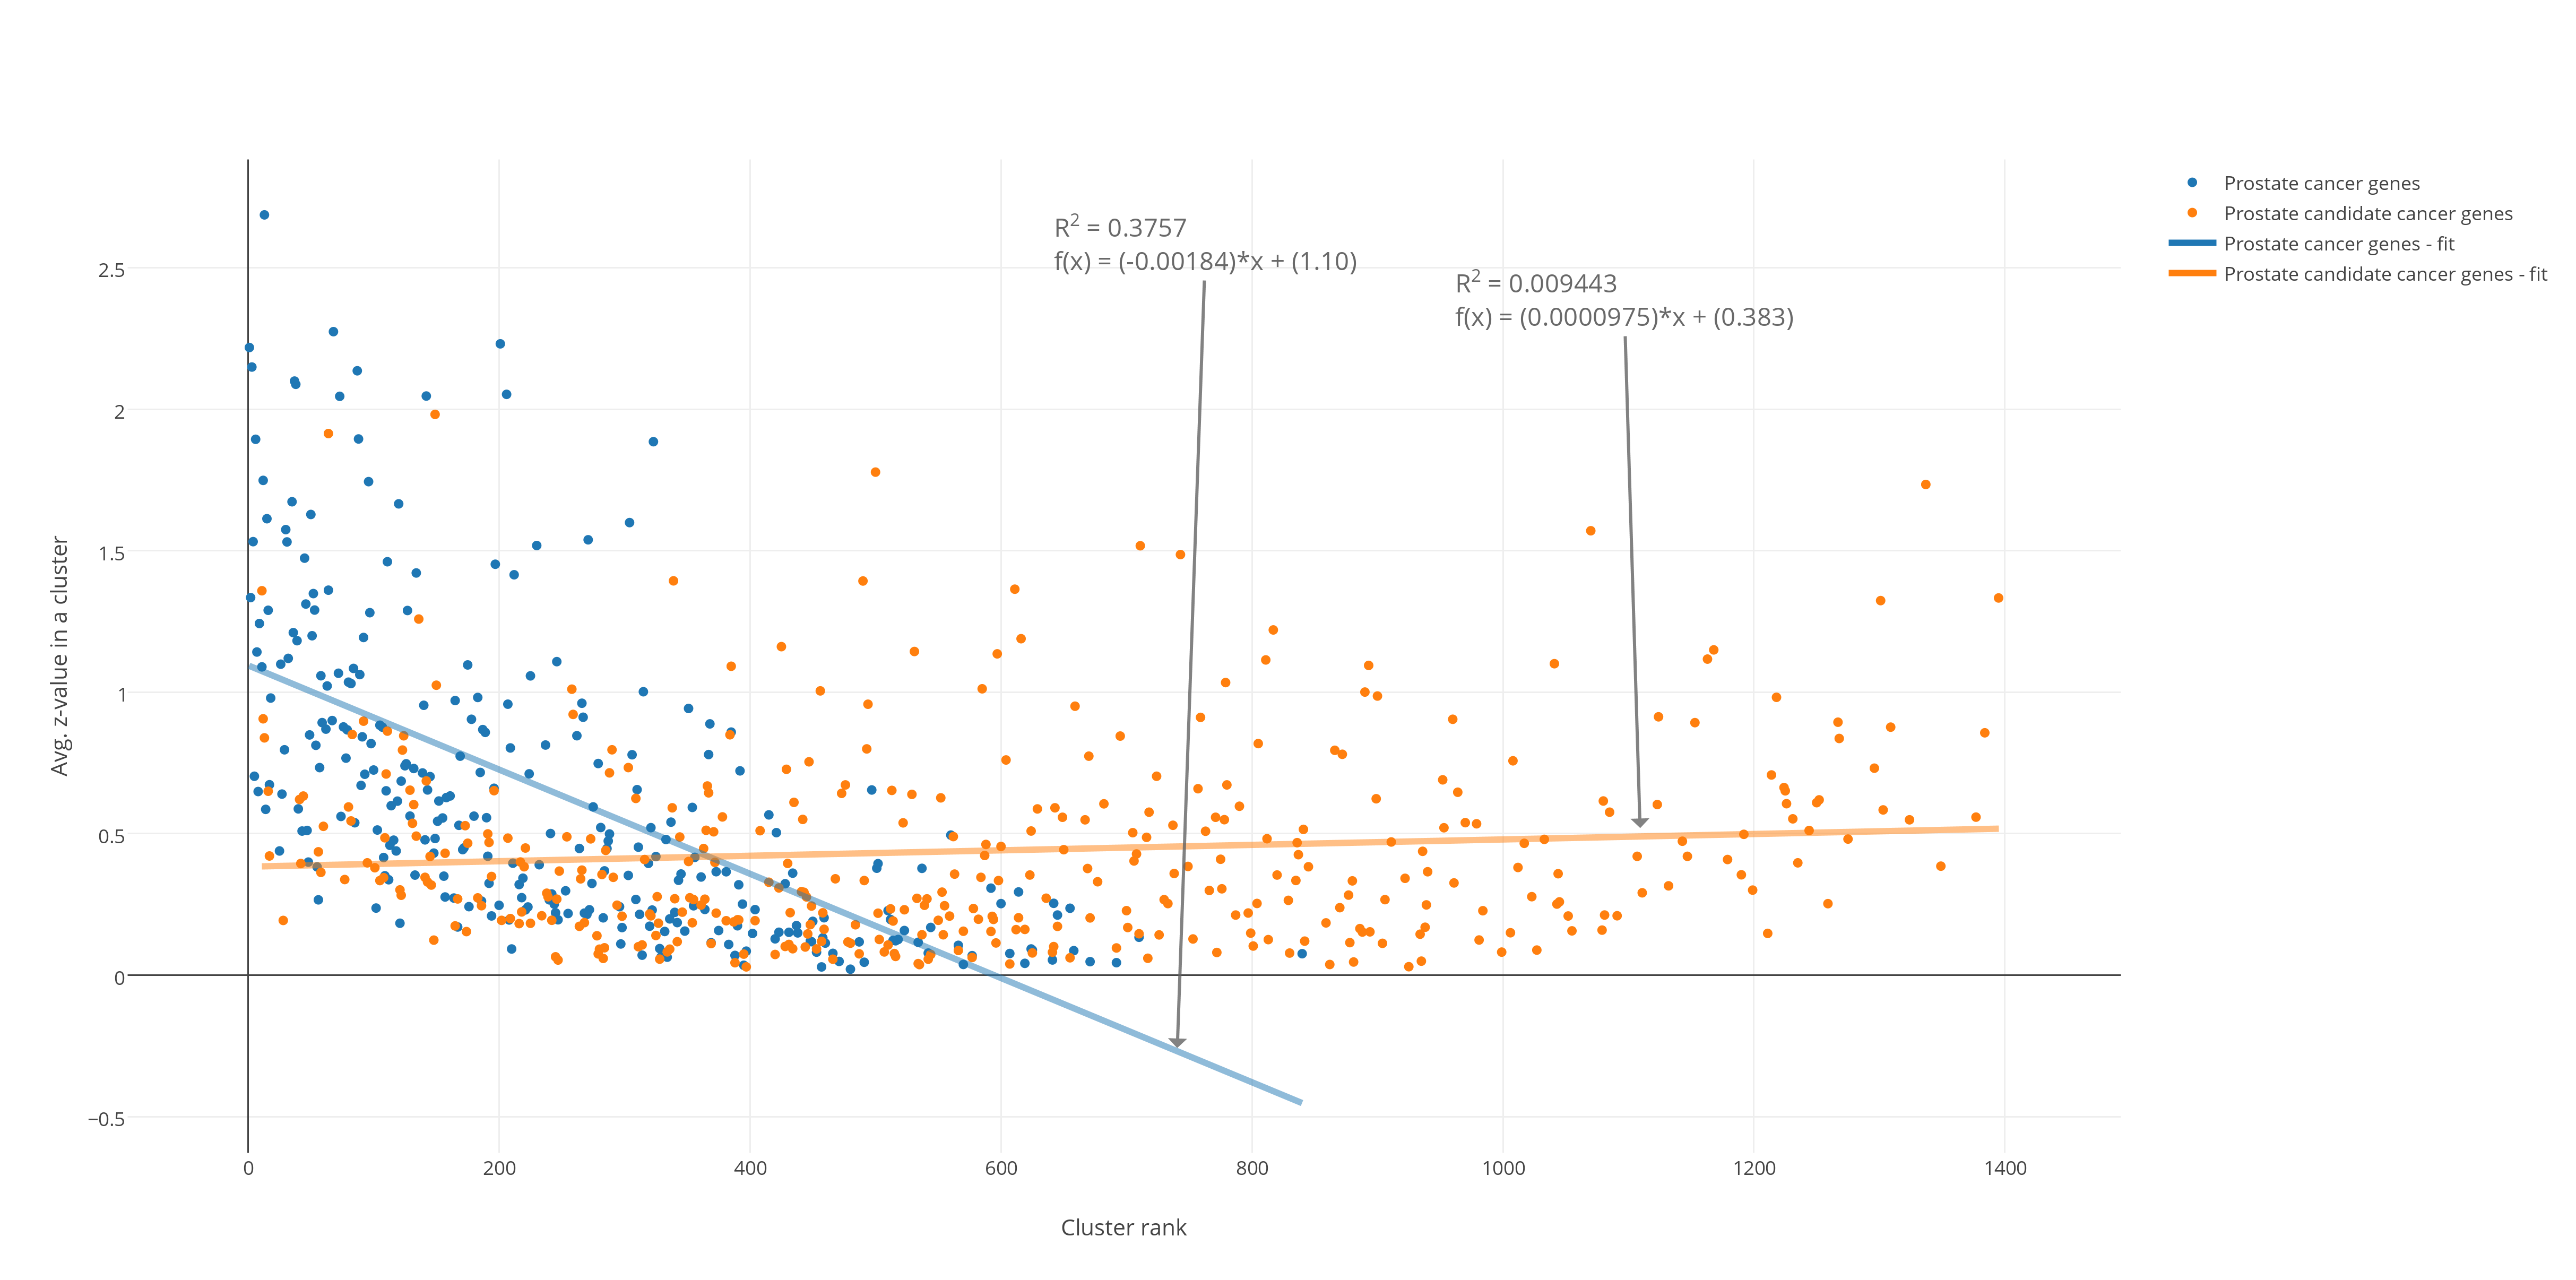
\includegraphics[width=15cm]{prwp_txt_split}
    \caption{Average distribution of z-scores in clusters ranked by PRWP.}
\end{figure}
For \gls{prwp}, the prostate cancer candidate genes is descending in z-values
from the topmost ranked cluster to the lowest, which is contributing to
showing \gls{prwp}s suitability for ranking clusters as candidate biomarkers. 

The prostate candidate cancer biomarkers are ascending in z-value from the
topmost to the lowest ranked cluster. High z-values would contribute to the fact
that ranklust has found actual prostate candidate cancer biomarkers. However,
a low z-values does not contradict it. The only fact to deduce from low z-values
is that they have not been examinated to the degree that they are not mentioned
in papers related to prostate cancer.

\begin{figure}[H]
    \label{fig:txt-iref-maa}
    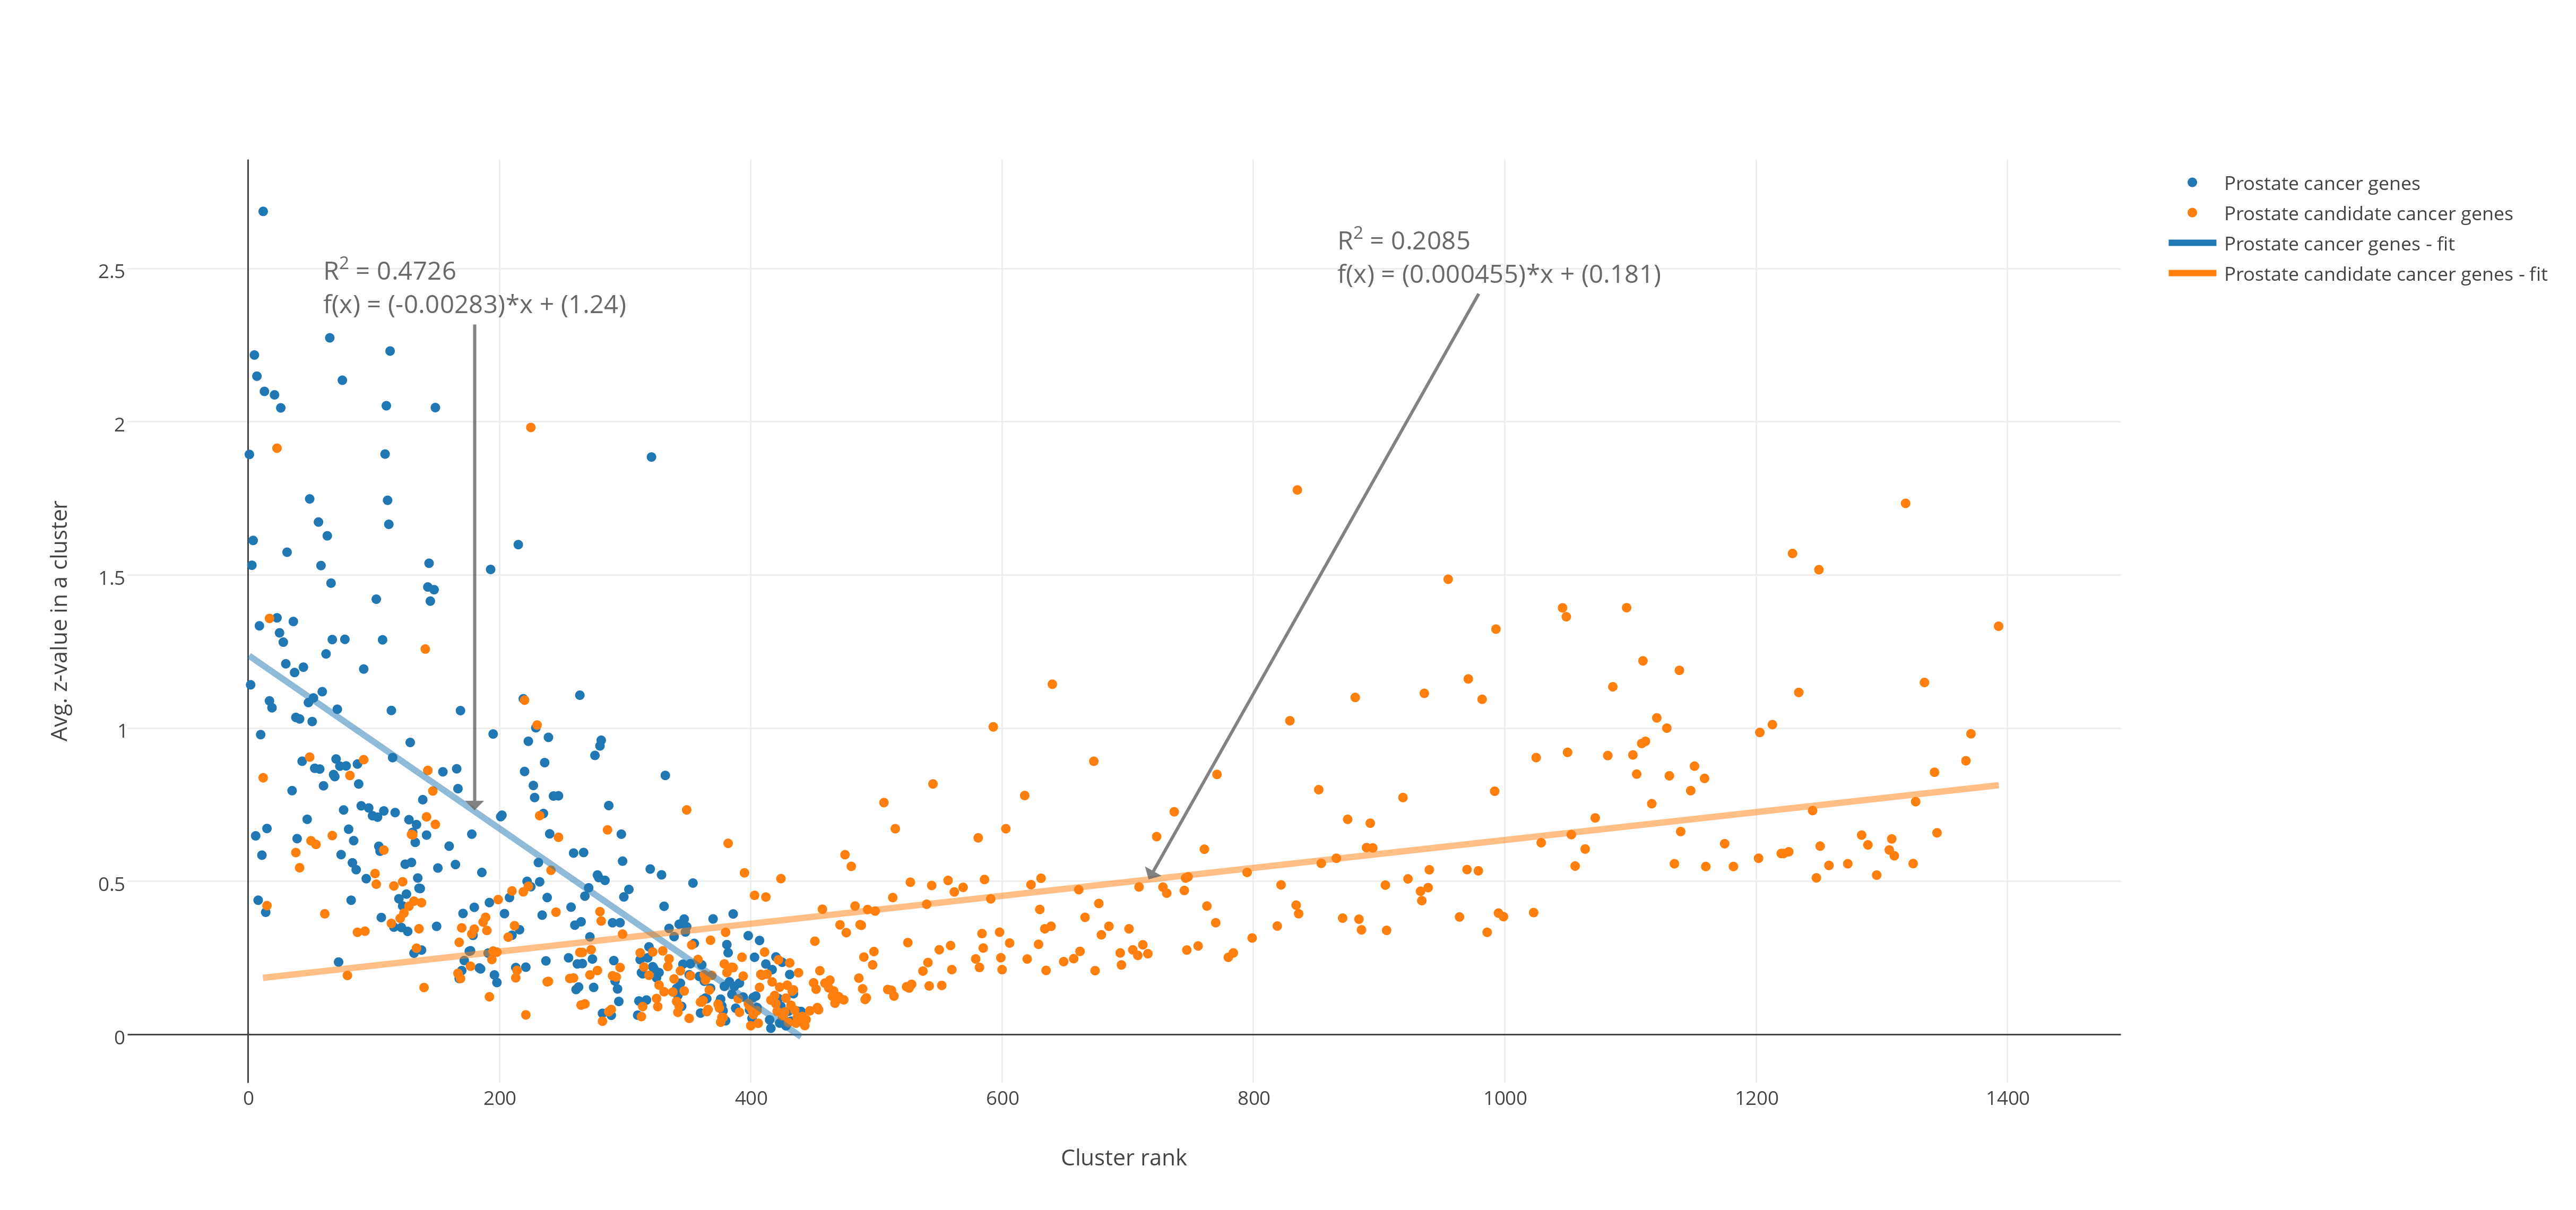
\includegraphics[width=15cm]{maa_txt_split}
    \caption{Average distribution of z-scores in clusters ranked by MAA.}
\end{figure}
For \gls{maa}, the prostate cancer genes have the same distinct descension in
z-values from the topmost to the lowest cluster ranks. The difference from
\gls{prwp} to \gls{maa} being that \gls{maa} has a more distinct ascending
linear regresstion fit for the z-values in the prostate candidate cancer genes.

This demonstrates the main difference between \gls{prwp} and \gls{maa}.
\gls{prwp} takes network structure into comparison as well as the prior scores.
\gls{maa} focuses purely on the prior scores, and so the network structure of
protein complexes are being completely ignored.

\subsection{Knowledge curated distribution of genes}
This data had no score except for a confidence score in the \gls{jensen}
database. Due to the low grade of distinctiveness between the different genes in
the database, the average amount of genes in a cluster would receive a knowledge
score based on if the gene occurs in the knowledge curated part of the
\gls{jensen} database or not. So the knowledge curated data is only based on
occurence, and not a specific value, in contrast to the text mined and
experimentally mined genes in the database.

Another trait the knowledge curated data posssesses is the amount entries in the
\gls{jensen} database that has. Text mined data can be seen as the
high-throughput technology of retrieving relevant data from papers, while the
knowledge curated data is manually curated by researchers. This is why the
amount of entries for knowledge curated data is so low when compared to text
mined data.

\begin{figure}[H]
    \label{fig:know-iref-prwp}
    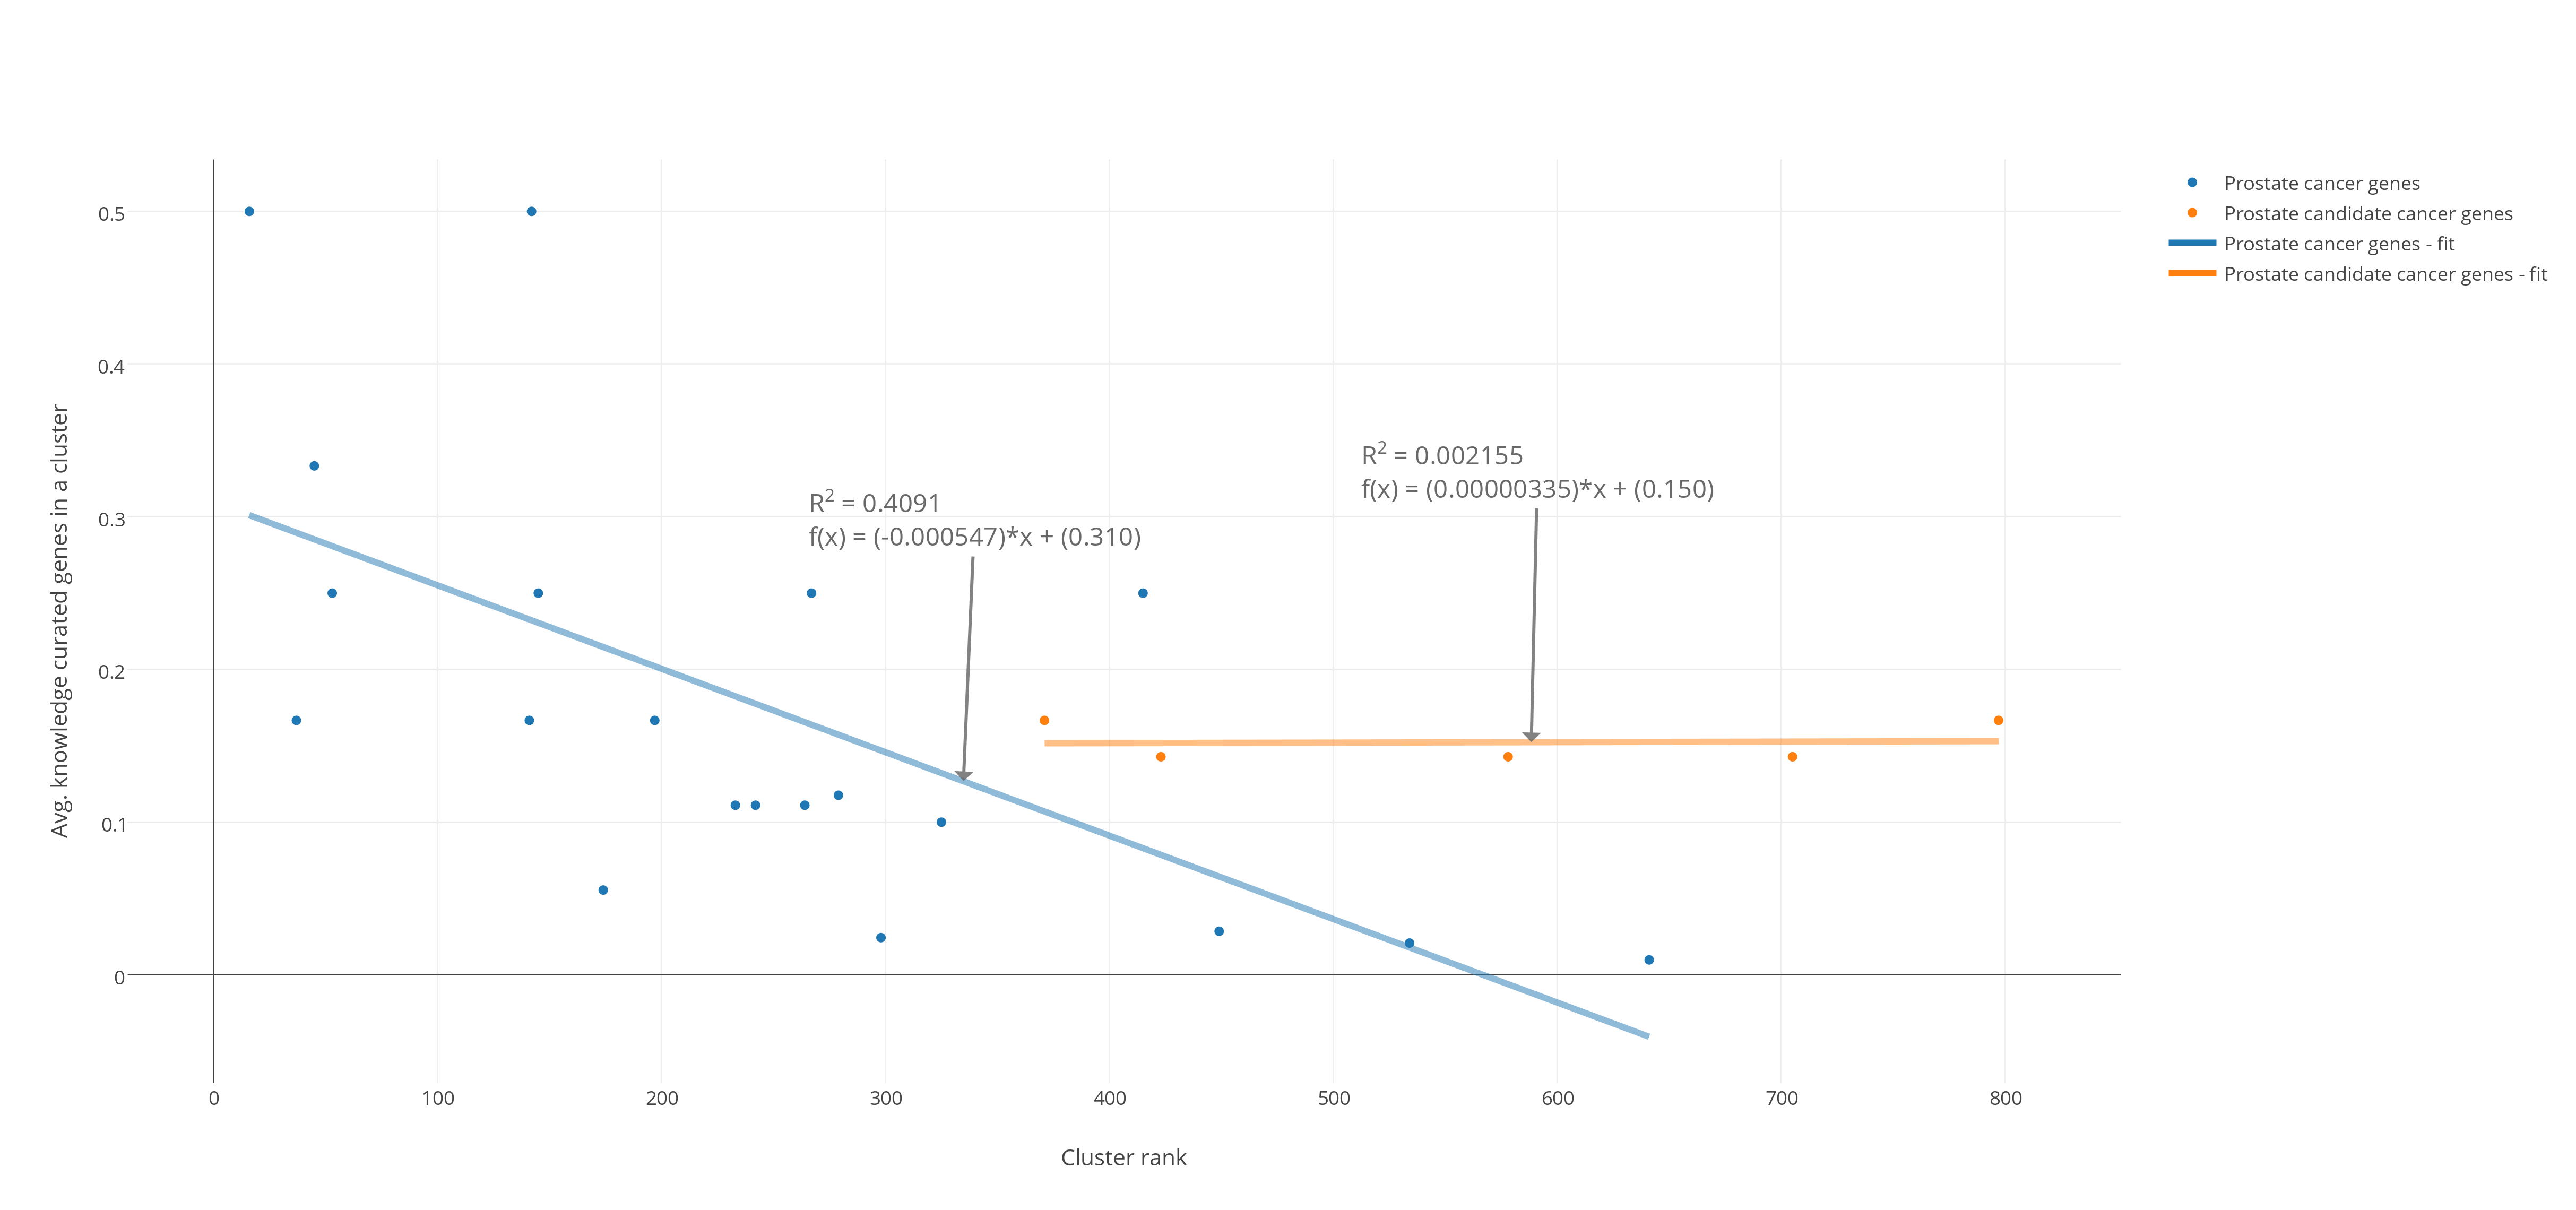
\includegraphics[width=15cm]{prwp_know_split}
    \caption{Average distribution of curated knowledge mined genes in clusters
    ranked by PRWP.}
\end{figure}
-- PRWP knowledge curated data discussion --

\begin{figure}[H]
    \label{fig:know-iref-maa}
    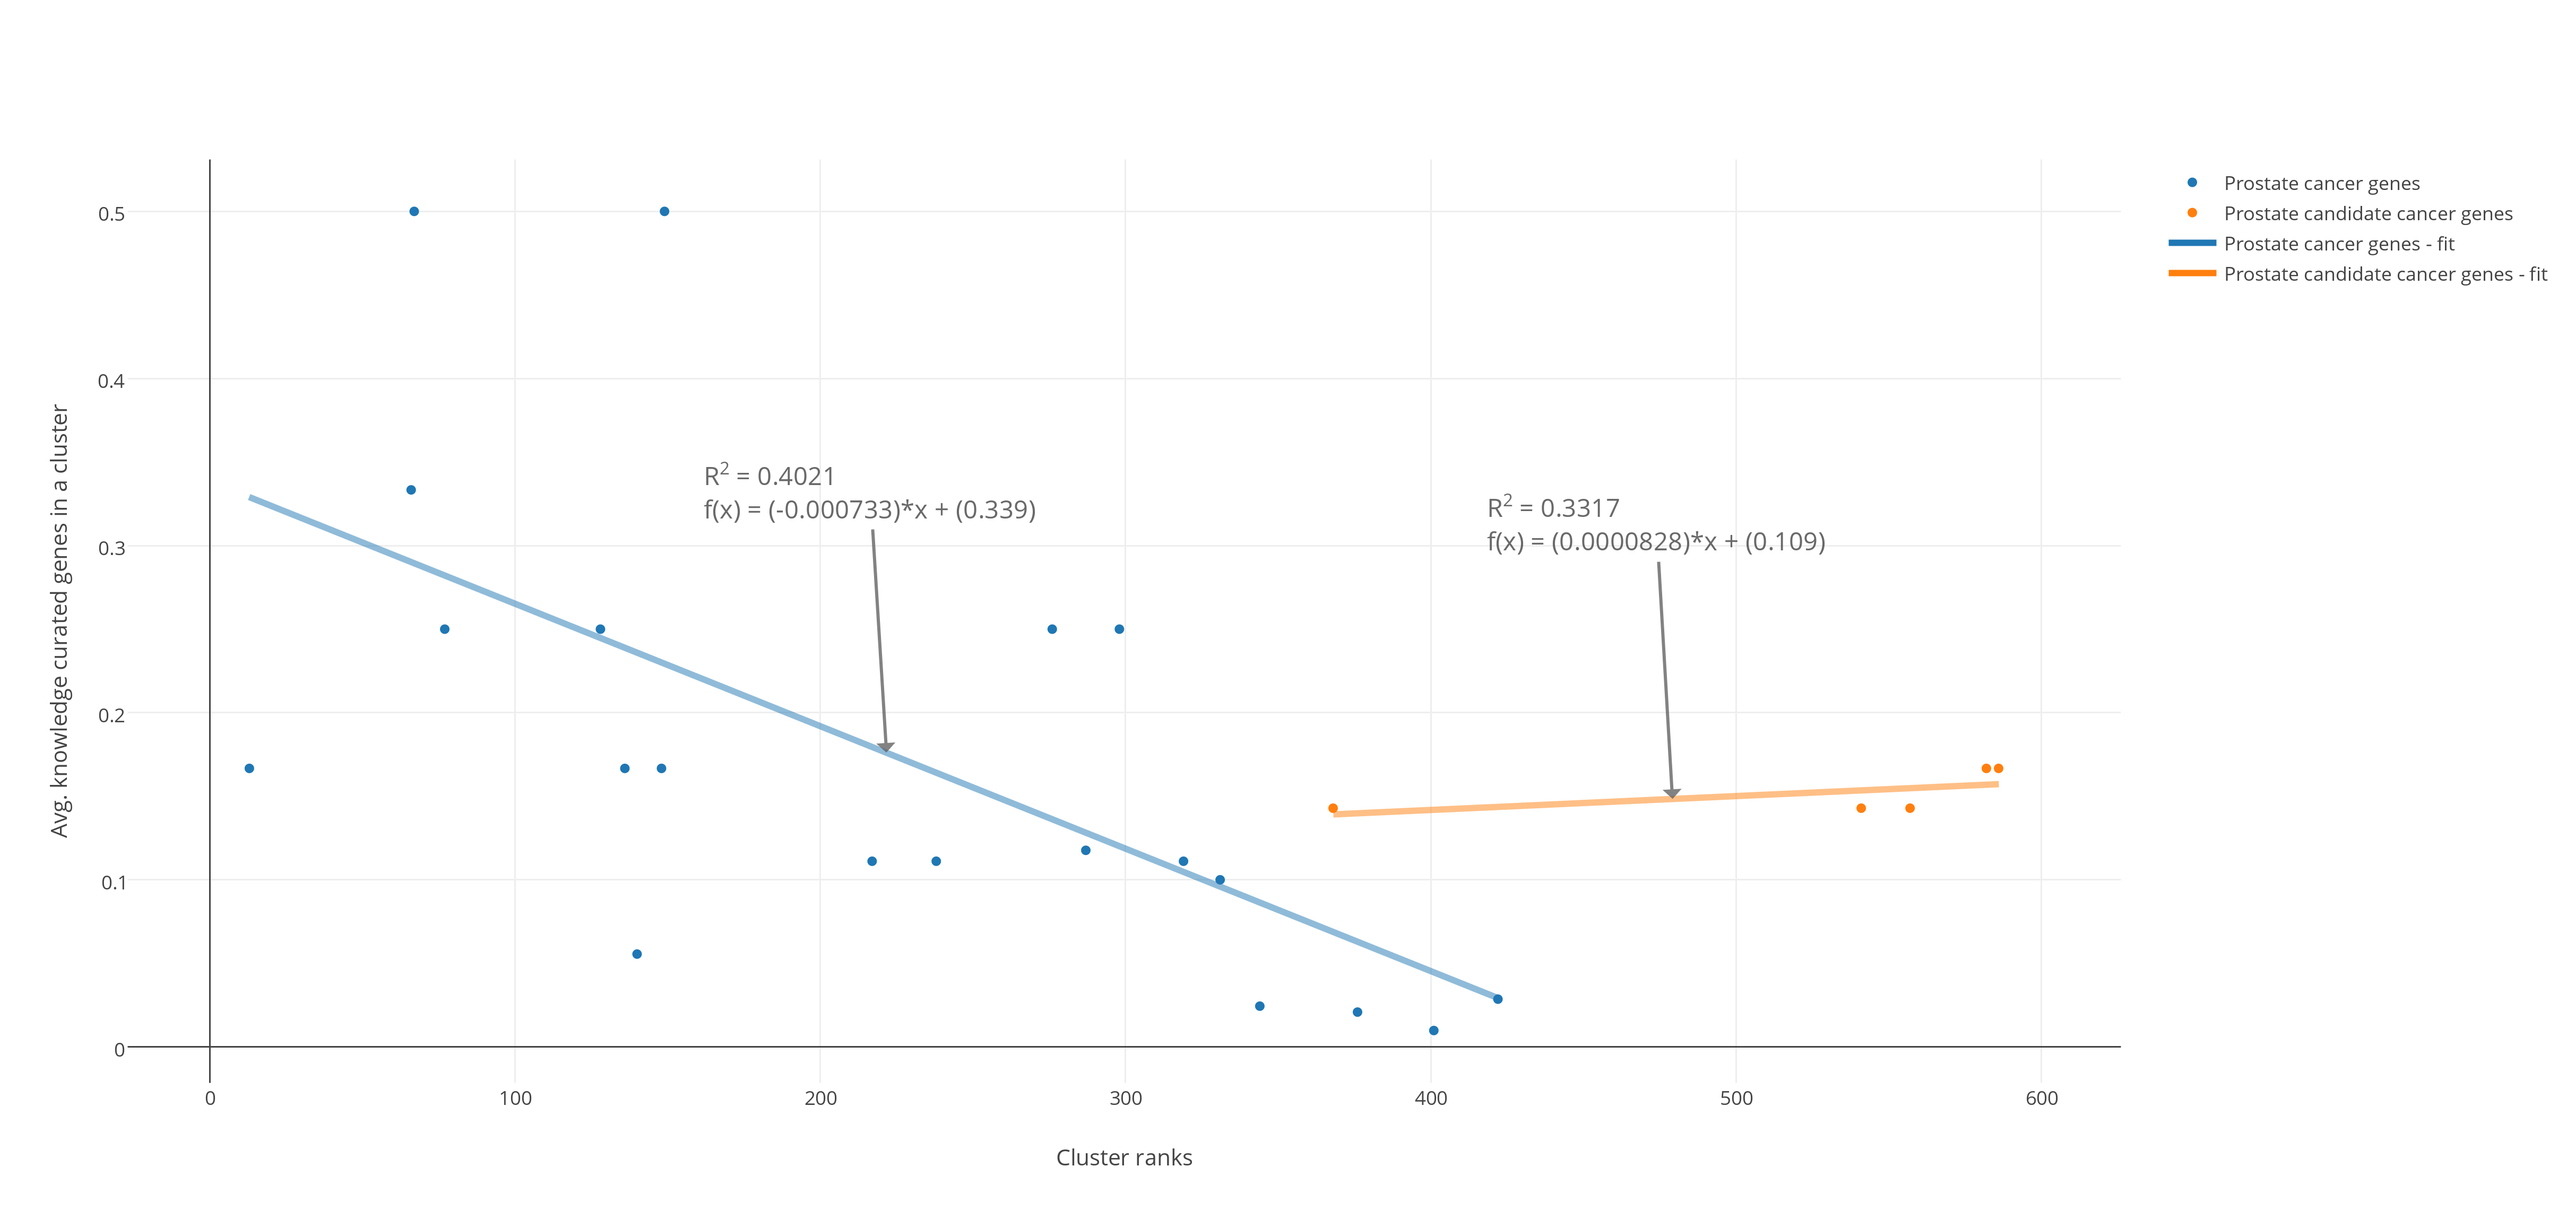
\includegraphics[width=15cm]{maa_know_split}
    \caption{Average distribution of curated knowledge mined genes in clusters
    ranked by MAA.}
\end{figure}
-- MAA knowledge curated data discussion --

\subsection{Experimental mined genes distribution of p-values in genes}
\begin{figure}[H]
    \label{fig:exp-iref-prwp}
    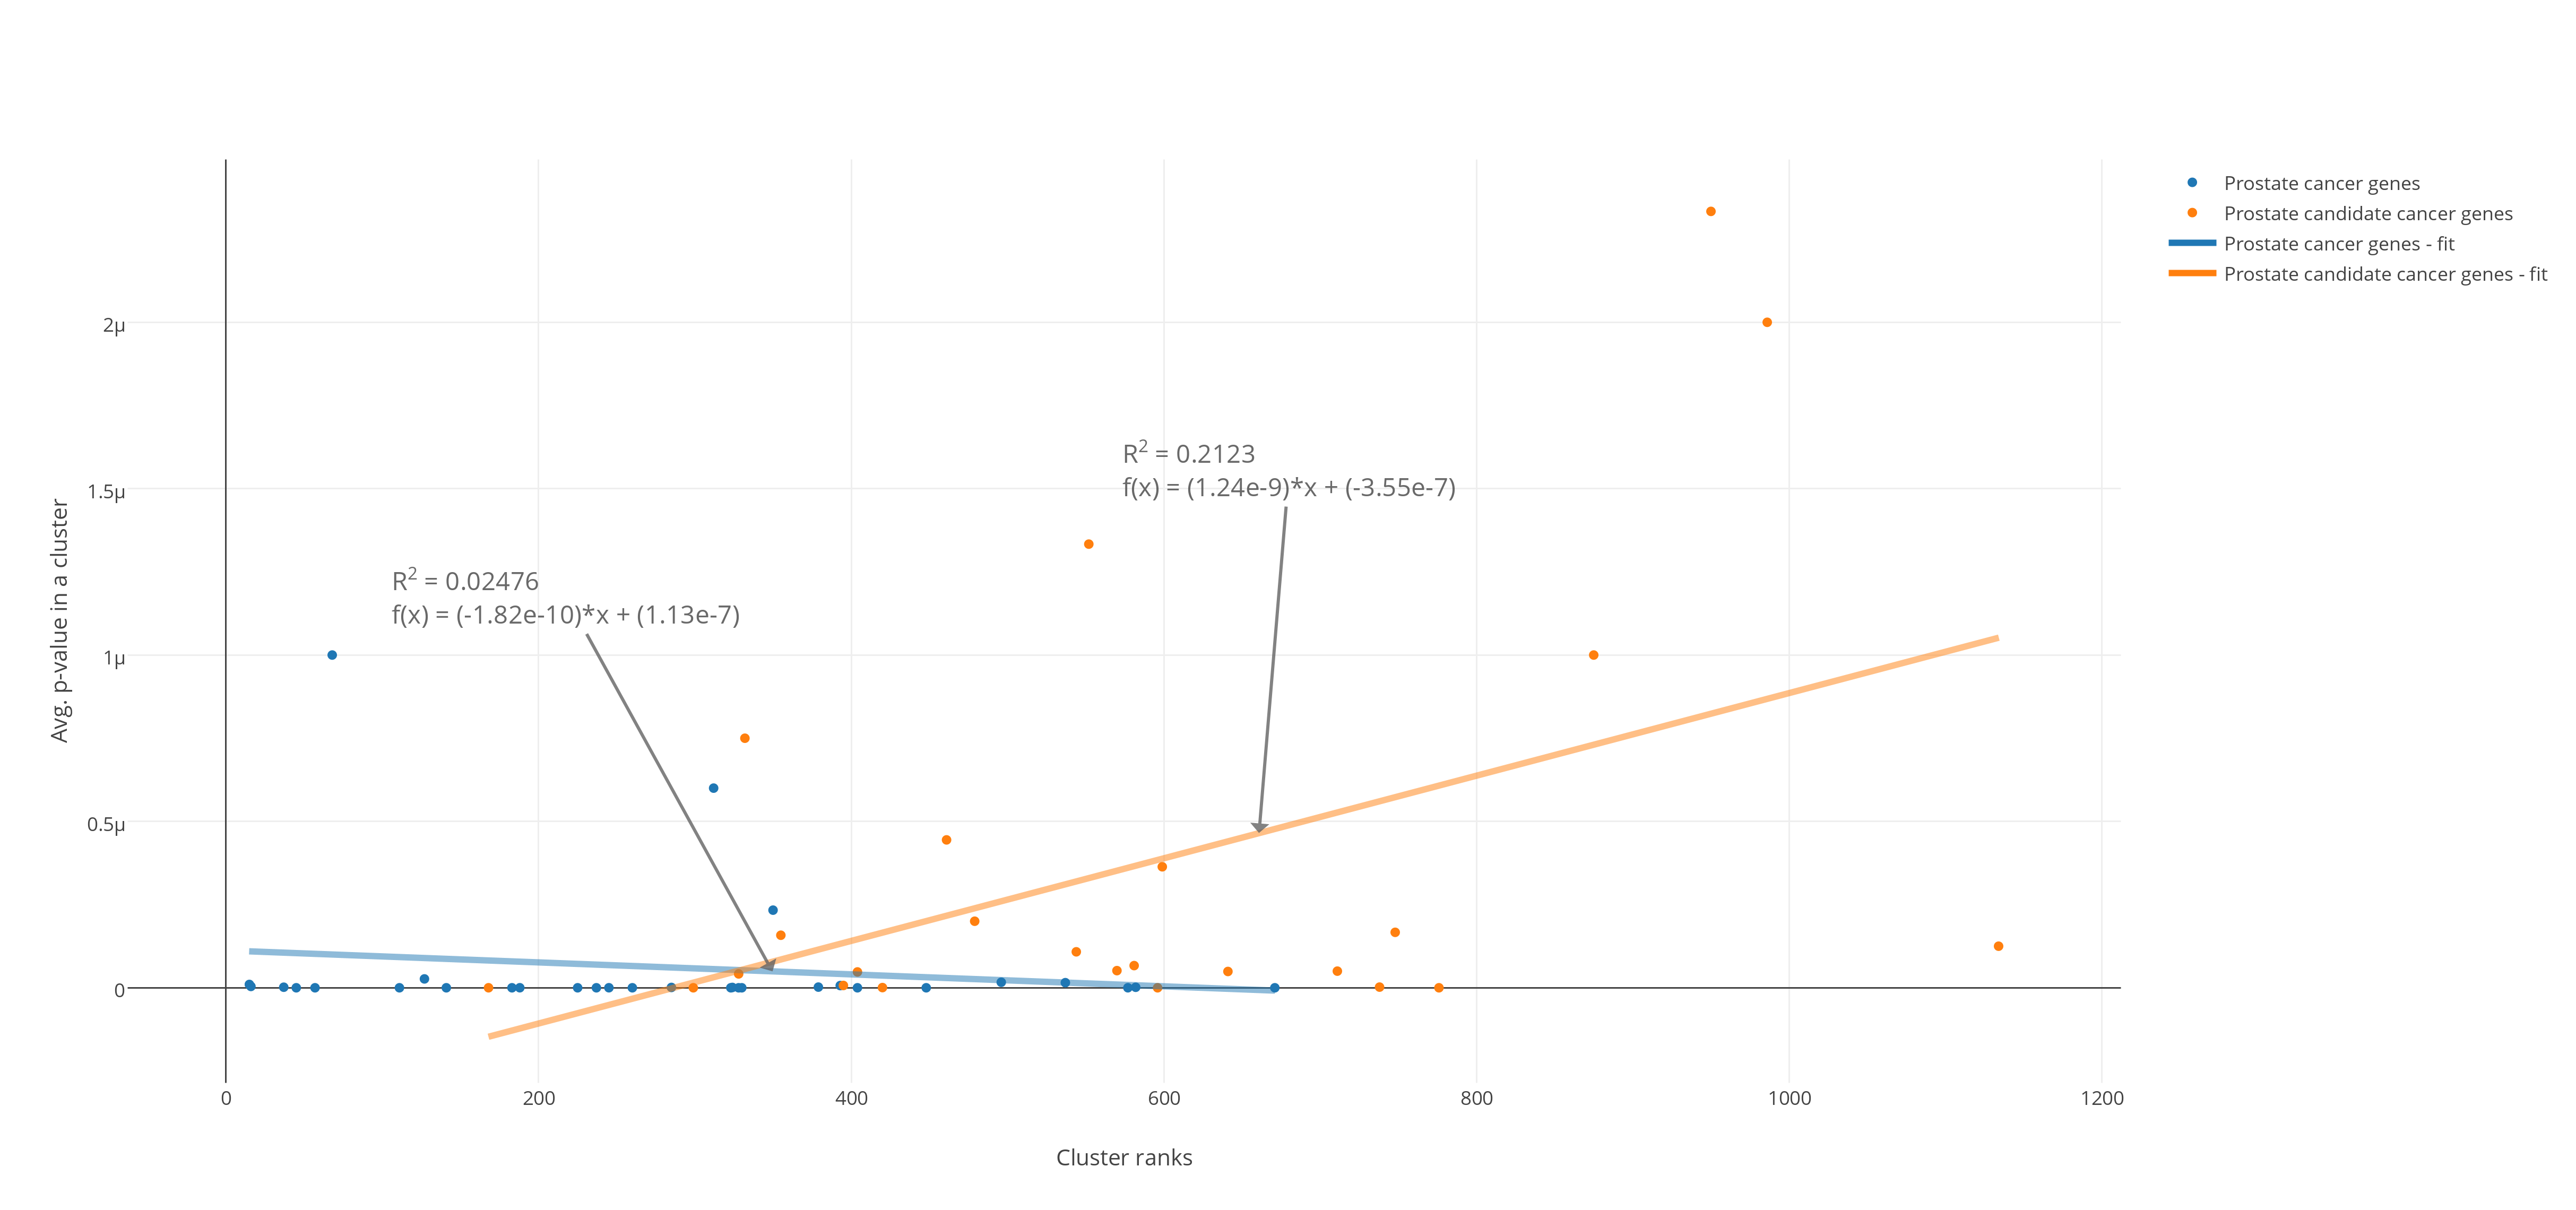
\includegraphics[width=15cm]{prwp_exp_split}
    \caption{Average distribution of p-values in clusters ranked by PRWP.}
\end{figure}
-- PRWP experimentally mined data discussion --

\begin{figure}[H]
    \label{fig:exp-iref-maa}
    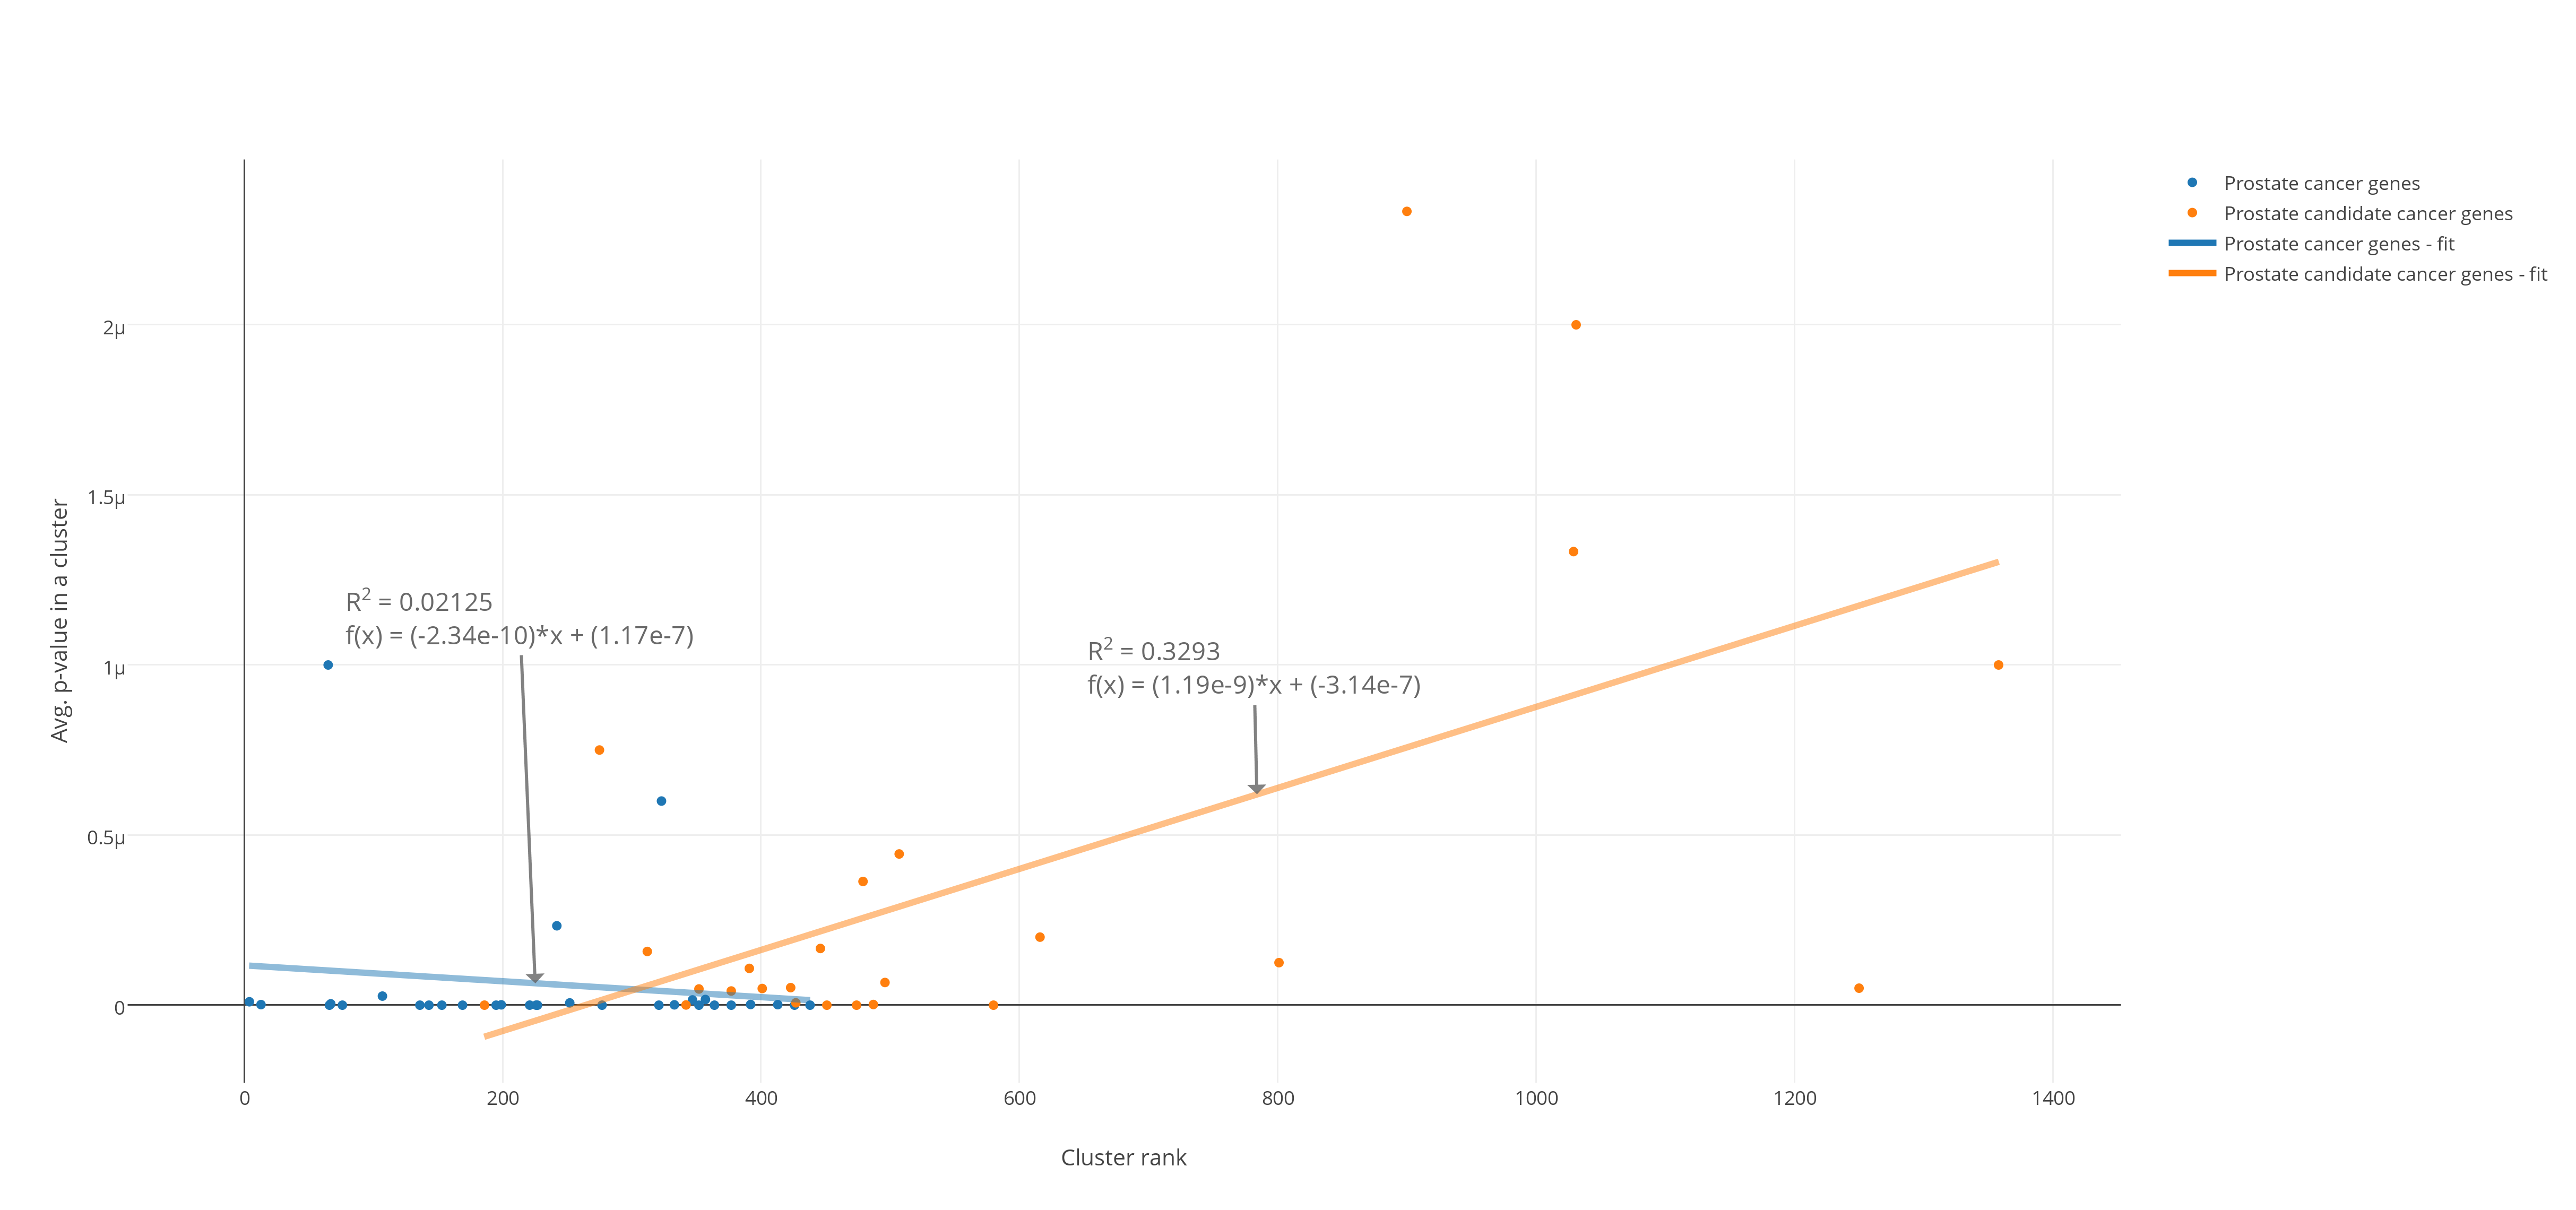
\includegraphics[width=15cm]{maa_exp_split}
    \caption{Average distribution of p-values in clusters ranked by MAA.}
\end{figure}
-- MAA experimentally mined data discussion --


\section{Comparison to known biomarkers}
-- Tests from Movember data etc. --

\section{Identification of possible cluster biomarkers}
-- Final list with cluster biomarkers --
\begin{table}
    \begin{tabular}{|p{1cm}|p{3cm}|p{3cm}|p{4cm}|}
        \hline
        \textbf{Rank} & \textbf{Biomarkers} & \textbf{Candidates} & \textbf{Remaining} \\
        \hline
        13	& TNFRSF11B	& THBS1	& VEGFA \\
        \hline
        19	& -	& F12	& MMP12 \\
        \hline
        25	& F2R	& -	& F2RL1, PRTN3 \\
        \hline
        28	& -	& RRM2	& MAGEA3, DNM1L, MAGEA1, PGAM5, SCG3 \\
        \hline
        29	& CEACAM1	& -	& CLEC4M \\
        \hline
        31	& ALOX15B	& -	& ERAL1 \\
        \hline
        46	& SMAD4	& -	& ZMIZ1 \\
        \hline
        48	& STAT6	& -	& ACSL3, IFI16, TRIM56, TMEM173, SLC39A14 \\
        \hline
        53	& RNASEL	& IQGAP1	& GSPT1, NPHS2 \\
        \hline
        55	& DPP4	& -	& PYY, GHRH, GCG, GIP, TAC1, FAP, VIP, AVPR1A, ADCYAP1, NPPB \\
        \hline
        58	& MMP9	& -	& CXCL1, HAPLN1, CXCL2, MMP10, MMP26 \\
        \hline
        60	& -	& KPNA2	& TXNIP, APOBEC1 \\
        \hline
        67	& PIN1	& -	& RUNX2, PPM1D, SULT4A1, GPHN \\
        \hline
        73	& CD44	& -	& SCYL3 \\
        \hline
        76	& MUC1	& -	& HPX, APOB, ORM1, LGALS9, LGALS8, ITGAL, LGALS3, A1BG \\
        \hline
        78	& NRP1	& -	& PLXNA2, PLXNA1, NRP2, VEGFC, VEGFD \\
        \hline
        79	& BIRC5	& -	& KCNJ6 \\
        \hline
        88	& SERPINA3	& -	& CTRC, GZMM, SGCD, KLK4 \\
        \hline
        91	& -	& CRIP2	& NR1H4, NME5, UXT, RELA, ALPL \\
        \hline
        92	& CCNB1	& UBE2C	& UBE3D \\
        \hline
    \end{tabular}
    \caption{Network }
    \label{tab:prwp-movember}
\end{table}
